\documentclass[fleqn]{NotesClass}

%% Packages
\usepackage{csquotes}
\usepackage{cancel}

% Tikz stuff
\usepackage{tikz}
\tikzset{>=latex}
% £xternal
\usetikzlibrary{external}
\tikzexternalize[prefix=tikz-external/]
%\tikzexternaldisable
% Other libraries
\usetikzlibrary{angles}
\usetikzlibrary{quotes}
\usetikzlibrary{3d}

% References, should be last things loaded
\usepackage{hyperref}  % Should be loaded second last (cleveref last)
\colorlet{hyperrefcolor}{blue!60!black}
\hypersetup{colorlinks=true, linkcolor=hyperrefcolor, urlcolor=hyperrefcolor}
\usepackage[
capitalize,
nameinlink,
noabbrev
]{cleveref} % Should be loaded last

% My packages
\usepackage{NotesBoxes}
\usepackage{NotesMaths}


% Title page info
\title{Lagrangian Dynamics}
\author{Willoughby Seago}
\date{September 20, 2021}
% \subtitle{}
% \subsubtitle{}

% Highlight colour
\definecolor{highlight}{HTML}{255029}
\definecolor{complementaryteal}{HTML}{254C50}
\definecolor{complementarypurple}{HTML}{50254C}
\definecolor{complementaryred}{HTML}{502925}
%% Commands
% Text


% Maths
\newcommand*{\e}{\mathrm{e}}
\newcommand*{\vedot}[1]{\dot{\vv{e}}_{\vv{#1}}}
\newcommand*{\eff}{\mathrm{eff}}
\newcommand*{\order}{\mathcal{O}}
\newcommand*{\ext}{\mathrm{ext}}
\newcommand*{\constraint}{\mathrm{constraint}}
\newcommand*{\other}{\mathrm{other}}
\newcommand*{\nodependence}[1]{\textcolor{gray}{\cancel{#1}}}
\newcommand*{\lagrangian}{\mathcal{L}}

% Include
\includeonly{parts/appendix-odes}

\begin{document}
    \frontmatter
    \titlepage
    \innertitlepage{tikz-external/effective-central-potential.pdf} 
    \tableofcontents
    \mainmatter
    \chapter{Introduction}
    The Lagrangian formalism of classical mechanics was pioneered by Joseph-Louis Lagrange.
    It is an alternative to Newton's formulation of classical mechanics.
    In many ways it is more powerful than Newton's formulation.
    For example, the Lagrangian formalism can easily include constraints on the system and is readily adapted to apply to electromagnetism, quantum mechanics, and relativistic systems.
    A task which is either impossible or incredibly difficult for the Newtonian formalism.
    Another benefit is that the Lagrangian formalism is built upon scalar quantities, which are often easier to work with than vectors.
    
    \part{Preparing for the Lagrangian Formalism}
    \chapter{Newton's Laws and Conservation Laws}
    \section{Newton's Laws}
    Newtonian mechanics is based on Newton's laws, a set of three laws that combined allow us to describe mechanics at everyday scales, that is when things are: not too fast (so no need for special relativity), not too massive (so no need for general relativity), and not too small (so no need for quantum mechanics).
    
    Before we can state Newton's laws we will need a few bits of notation and basic definitions.
    For now we consider point like particles and measure their position relative to some origin, \(O\).
    \begin{ntn}{Basic Quantities}{}
        \begin{itemize}
            \item \(\vv{r}\) denotes the position vector.
            \item \(\vv{v}\) denotes the velocity vector.
            \item \(\vv{a}\) denotes the acceleration vector.
            \item \(\vv{p}\) denotes the linear momentum vector.
            \item Given some differentiable quantity, \(f\), we denote by \(\dot{f}\) the total time derivative, \(\diff{f}/{t}\), and by \(\ddot{f}\) the second total time derivative, \(\diff[2]{f}/{t}\).
            We should not have use of higher time derivatives but if we do then the it should be clear how this dot notation generalises.
        \end{itemize}
    \end{ntn}
    
    \begin{dfn}{Basic Quantities}{}
        \begin{itemize}
            \item The \defineindex{velocity} is defined by \(\vv{v} \coloneqq \dot{\vv{r}}\).
            \item The \defineindex{acceleration} is defined by \(\vv{a} = \dot{\vv{v}} = \ddot{\vv{r}}\).
            \item The \define{momentum}\index{momentum!linear} is defined by \(\vv{p} = m\vv{v}\).
        \end{itemize}
    \end{dfn}
    
    We can now state Newton's laws.
    \paragraph{N1} \defineindex{Newton's first law} (N1)\glossary[acronym]{N1}{Newton's first law} states that in the absence of forces \(\vv{v}\) is constant.
    \paragraph{N2} \defineindex{Newton's second law} (N2)\glossary[acronym]{N2}{Newton's second law} states that in the presence of a force, \(\vv{F}\), the rate of change of linear momentum is \(\dot{\vv{p}} = \vv{F}\).
    A special case of this is when the mass is constant, which we will assume unless stated otherwise, in which case we recover the famous
    \begin{equation}
        \dot{\vv{p}} = m\dot{\vv{v}} = m\vv{a} = \vv{F}.
    \end{equation}
    In Newtonian mechanics we start most problems by assuming that the force, \(\vv{F}\) is either known or can be easily found.
    We then solve N2 for the equations of motion.
    \paragraph{N3} \defineindex{Newton's third law} (N3)\glossary[acronym]{N3}{Newton's third law} comes in two forms, a weak form and a strong form.
    In both we consider the force \(\vv{F_{ab}}\), which is the force on particle \(a\) due to particle \(b\).
    The weak form states that \(\vv{F_{ab}} = -\vv{F_{ba}}\).
    The strong form states that as well as this \(\vv{F_{ab}}\) is directed along \(\vv{r_{ab}} = \vv{r_a} - \vv{r_b}\) where \(\vv{r_a}\) is the position of \(a\) and \(\vv{r_b}\) the position of \(b\).
    
    \subsection{Caveats}
    Newton's laws all come with caveats.
    Obviously, due to the need for quantum mechanics and relativity, Newton's laws aren't always valid.
    So, we need to be careful about when we apply them.
    
    N1 and N2 are only valid in non-accelerating frames, that is when there are no external forces.
    We call these \define{inertial frames}\index{inertial frame}.
    We typically assume frames are inertial unless stated otherwise.
    Apart from linearly accelerating frames it should be noted that rotating frames aren't inertial, even for a constant rotation speed.
    This, as well as the movement around the sun, and movement of the solar system, and movement of the solar system, and the movement of the galaxy and, \dots, means that the Earth is \emph{not} an inertial frame.
    However, it is a sufficiently good approximation of an inertial frame for most of our everyday requirements.
    There are a few cases, such as Foucault's pendulum, where the rotation of the Earth has a non-negligible effect.
    
    Both forms of N3 only hold for types of force.
    For example, since the force from a magnetic field is orthogonal to the velocity, means that in general the strong form of N3 doesn't hold for charged particles.
    
    \section{Conservation Laws}
    Conservation laws are \emph{incredibly} important in physics.
    One advantage of the Lagrangian formalism is how easy it is to find conservation laws with it.
    However, for now we restrict our selves to deriving the most important conservation laws from the Newtonian formalism.
    
    \subsection{Conservation of Linear Momentum}
    Suppose there is no force, so \(\vv{F} = \vv{0}\).
    It immediately follows from N2 that \(\dot{\vv{p}} = \vv{F} = \vv{0}\) and hence \(\vv{p}\) is constant.
    We say that in the absence of external forces linear momentum is conserved.
    A consequence of this is that if \(m\) is a constant then \(\vv{a} = \vv{0}\) and so the particle travels at a constant velocity.
    
    \subsection{Conservation of Angular Momentum}
    \begin{dfn}{Angular Momentum and Torque}{}
        For a particle at position \(\vv{r}\) and linear momentum \(\vv{p}\) we define its \define{angular momentum}\index{momentum!angular} with respect to the origin to be
        \begin{equation}
            \vv{L} \coloneqq r\times \vv{p}.
        \end{equation}
        If a force, \(\vv{F}\), is applied to the particle then we define the \defineindex{torque}, also known as the \defineindex{moment of force} about the origin to be
        \begin{equation}
            \vv{G} \coloneqq \vv{r} \times \vv{F}.
        \end{equation}
    \end{dfn}
    Note that since they are defined via cross products both \(\vv{L}\) and \(\vv{G}\) are axial vectors (aka pseudovectors), meaning that if we change between a left and right handed coordinate system then these vectors change sign.
    
    Applying N2 to the definition of torque we have
    \begin{equation}
        \vv{G} = \vv{r}\times\vv{F} = \vv{r}\times\dot{\vv{p}} = \diff*{(\vv{r}\times\vv{p})}{t} - \dot{\vv{r}}\times\vv{p}
    \end{equation}
    where in the last step we have used the chain rule:
    \begin{equation}
        \diff*{(\vv{r}\times\vv{p})}{t} = \vv{r}\times\dot{\vv{p}} + \dot{\vv{r}}\times\vv{p} \implies \vv{r}\times\dot{\vv{p}} = \diff*{(\vv{r}\times\vv{p})}{t} - \dot{\vv{r}}\times\vv{p}.
    \end{equation}
    We now look at this last term, \(\dot{\vv{r}}\times\vv{p}\), in more detail.
    Noticing that \(\dot{\vv{r}} =\vv{v}\) and \(\vv{p} = m\vv{v}\) we see that this term is zero, since the cross product of any two collinear vectors is zero.
    Hence,
    \begin{equation}
        \vv{G} = \diff*{(\vv{r}\times\vv{p})}{t} = \dot{\vv{L}}
    \end{equation}
    where we have used the definition of angular momentum, \(\vv{L} = \vv{r}\times\vv{p}\).
    From this we see that if \(\vv{G} = \vv{0}\) then \(\dot{\vv{L}} = \vv{0}\) and hence \(\vv{L}\) is constant.
    We say that in the absence of external torques angular momentum is conserved.
    
    \subsection{Conservation of Energy}
    \begin{dfn}{Work Done}{}
        The \defineindex{work done} to move a particle along a path, \(\Gamma\), requiring force \(\vv{F}\) is defined as
        \begin{equation}
            W\coloneqq \int_\Gamma \vv{F}\cdot\dl{\vv{r}}.
        \end{equation}
    \end{dfn}
    
    Consider the work done to move a particle from \(A\) to \(B\) along some path, which we parametrise as a function of \(t\) (which may or may not be time) such that when \(t = t_A\) the particle is at \(A\) and when \(t = t_B\) the particle is at \(B\).
    We will assume a constant mass but the following result holds for a variable mass, the derivation is just more involved.
    \begin{align}
        W_{AB} &= \int_A^B \vv{F}\cdot\dl{\vv{r}}\\
        &= \int_{t_A}^{t_B} \vv{F} \cdot\diff{\vv{r}}{t}\dd{t}\\
        &= \int_{t_A}^{t_B} \dot{\vv{p}}\cdot\vv{v}\dd{t}\\
        &= \int_{t_A}^{t_B} m\dot{\vv{v}}\cdot\vv{v}\dd{t}\\
        &= \frac{m}{2}\int_{t_A}^{t_B} v^2 \dd{t}\\
        &= \frac{m}{2}[v^2]_{t_A}^{t_B}\\
        &= \frac{1}{2}m[v(t_B)]^2 - \frac{1}{2}[v(t_A)]^2\\
        &= T_{B} - T_{A}\label{eqn:W=Tb-Ta}
    \end{align}
    where \(T\coloneqq \frac{1}{2}mv^2\) defines the \defineindex{kinetic energy} in Newtonian mechanics.
    Note that about halfway through the calculation we used
    \begin{equation}
        \diff*{(\vv{v}\cdot\vv{v})}{t} = \vv{v}\cdot\dot{\vv{v}} + \dot{\vv{v}}\cdot\vv{v} = 2\dot{\vv{v}}\cdot\vv{v} \implies \dot{\vv{v}}\cdot\vv{v} = \frac{1}{2}\diff*{(\vv{v}\cdot\vv{v})}{t}.
    \end{equation}
    We can see from this that the work done on a particle is equal to the change in kinetic energy of the particle.
    
    \begin{dfn}{Conservative Force}{}
        The following are equivalent:
        \begin{itemize}
            \item The force \(\vv{F}\) is \define{conservative}\index{conservative force}.
            \item The work done to move a particle from \(A\) to \(B\) is independent of the path taken, that is
            \begin{equation}
                \int_\Gamma \vv{F}\cdot\dl{\vv{r}} = \int_\gamma \vv{F}\cdot\dl{\vv{r}}
            \end{equation}
            where \(\Gamma\) and \(\gamma\) are two paths from \(A\) to \(B\).
            \item The following holds
            \begin{equation}
                \oint \vv{F}\cdot\dl{\vv{r}} = 0
            \end{equation}
            where \(\oint\) denotes an integral over a closed path, that is a path that starts and ends at the same point.
            \item There exists a scalar function, \(V\), such that
            \begin{equation}
                \vv{F} = -\grad V.
            \end{equation}
            \item The following holds
            \begin{equation}
                \curl\vv{F} = \vv{0}.
            \end{equation}
        \end{itemize}
    \end{dfn}
    
    Suppose \(\vv{F}\) is a conservative force.
    Then we can write \(\vv{F} = -\grad V\) for some scalar function \(V\). The negative sign here is just a convention so that we can minimise the potential, instead of maximising, which better aligns with our intuition and the original definition of potentials before this more general notion.
    We can use this to redo the calculation above:
    \begin{align}
        W_{AB} = \int_{A}^{B}\vv{F}\cdot\dl{\vv{r}}\\
        &= -\int_A^B \grad V \cdot\dl{\vv{r}}\\
        &= -\int_A^B\dd{V}\\
        &= V_B - V_A\label{eqn:W=Vb-Va}
    \end{align}
    where \(V_A\) and \(V_B\) are the value of the potential at \(A\) and \(B\) respectively.
    Note here that we used
    \begin{equation}
        \int\grad V\cdot\dl{\vv{r}} = \int\dd{V}
    \end{equation}
    which is the three dimensional analogue of
    \begin{equation}
        \int \diff{f}{x}\dd{x} = \int\dd{f}
    \end{equation}
    
    Combining \cref{eqn:W=Tb-Ta,eqn:W=Vb-Va} we get
    \begin{equation}
        T_A + V_A = T_B + V_B
    \end{equation}
    we define \(E \coloneqq T + V\) to be the \defineindex{total energy} and since this equation holds for any two points \(A\) and \(B\) this shows that, for a conservative force, the total energy is conserved.
    Since most, but not all, forces we meet in classical mechanics are conservative this is a very useful property.
    
    \chapter{Orbits}
    In this section we apply Newton's laws and conservation laws to one of the systems that motivated their development: orbiting planets.
    More generally we will consider some particle moving in a central force field described by a \defineindex{central potential} \(V(\vv{r}) = V(r)\).
    Our goal is to find an equation for the radial velocity of an orbiting particle.
    
    \section{Central Force}
    Recall that a \defineindex{central force} is one which depends only on the magnitude, \(r\), of the position vector, \(\vv{r}\) and acts along the line to the origin: \(\vv{F}(\vv{r}) = F(r)\vh{r} = -\grad V(r)\).
    Here \(\vh{r} = \vv{r}/r\) is a unit vector in the direction of the position vector.
    
    \subsection{Momenta}
    Assuming that \(\vv{F} \ne \vv{0}\) linear momentum will not be conserved.
    We can easily calculate the torque:
    \begin{equation}
        \vv{G} = \vv{r}\times\vv{F} = \vv{r}\times\vh{r}F = \vv{0}
    \end{equation}
    since the cross product of two collinear vectors is identically zero.
    Since there is no torque the angular momentum, \(\vv{L}\), is conserved.
    In particular the magnitude of the angular momentum, \(L\), is a constant.
    We have that
    \begin{equation}
        \vv{r}\cdot\vv{L} = \vv{r}\cdot(\vv{r}\times\vv{p}) = 0
    \end{equation}
    since \(\vv{r}\times\vv{p}\) is perpendicular to \(\vv{r}\).
    What we have here is of the form \(\vv{r}\) dotted with a constant vector equals a constant.
    This defines a plane perpendicular to the constant vector.
    The physical interpretation of this is that the particle is constrained to motion in the plane with normal \(\vv{L}\) containing the origin.
    
    \subsection{Coordinates}
    Since the particle is constrained to a plane we work in cylindrical polar coordinates, \((r, \varphi, z)\), with the \(\vh{z}\)-axis perpendicular to the plane of motion.
    In these coordinates
    \begin{align}
        x &= r\cos\varphi,\\
        y &= r\sin\varphi,\\
        z &= z,
    \end{align}
    where \(r = \abs{\vv{r}} = \sqrt{x^2 + y^2}\).
    In the plane of motion \(z = 0\).
    
    We define two orthonormal basis vectors, \(\ve{r}\) and \(\ve{\varphi}\), which are parallel and perpendicular, respectively, to the position vector, \(\vv{r}\).
    At the point \((r, \varphi, z)\) these vectors are given in terms of the Cartesian unit vectors, \(\ve{x}\), \(\ve{y}\), and \(\ve{z}\), by
    \begin{align}
        \ve{r} &\coloneqq \hphantom{-}\cos\varphi\ve{x} + \sin\varphi\ve{y}\label{eqn:e_r definition}\\
        \ve{\varphi} &\coloneqq -\sin\varphi\ve{x} + \sin\varphi\ve{y}.
    \end{align}
    The position vector is then
    \begin{equation}
        \vv{r} = x\ve{x} + y\ve{y} = r\ve{r}.
    \end{equation}
    
    \subsection{Velocity}
    The velocity of the particle can be found by differentiating the position vector with respect to time:
    \begin{align}
        \vv{v} &= \dot{\vv{r}}\\
        &= \diff*{(r\ve{r})}{t}\\
        &= \dot{r}\ve{r} + r\vedot{r}
    \end{align}
    Notice that, unlike Cartesian unit vectors, the cylindrical unit vectors are time dependent\footnote{rather they're position dependent and the position is time dependent} and so we have a second term involving the derivative of the unit vector.
    We can easily work out what this is by differentiating \cref{eqn:e_r definition}:
    \begin{align}
        \vedot{r} &= \diff*{(\cos\varphi\ve{x} + \sin\varphi\ve{y})}{t}\\
        &= -\dot{\varphi}\sin\varphi\ve{x} + \dot{\varphi}\cos\varphi\ve{y}\\
        &= \dot{\varphi}\ve{\varphi}.
    \end{align}
    Substituting this into the velocity we have
    \begin{equation}
        \dot{\vv{r}} = \dot{r}\ve{r} + r\dot{\varphi}\ve{\varphi}.
    \end{equation}
    We can see from this that the radial velocity is \(v_r = \dot{r}\), and the tangential component of the velocity is \(v_\varphi = r\dot{\varphi}\).
    
    \textcolor{highlight}{Be careful}: \(\dot{r} = v_r\) is not the same as \(\abs{\dot{\vv{r}}} = v\) here, for example, if motion is in a circle then \(\dot{r} = 0\) but \(\dot{\vv{r}} \ne \ve{0}\).
    
    \subsection{Using Conservation Laws}
    We can calculate the angular momentum now:
    \begin{align}
        \vv{L} &= \vv{r}\times\vv{p}\\
        &= \vv{r}\times\dot{\vv{r}}m\\
        &= mr[\ve{r} \times (\dot{r}\ve{r} + r\dot{\varphi}\ve{\varphi})]\\
        &= \vv{0} + mr^2\dot{\varphi}\ve{r}\times\ve{\varphi}\\
        &= mr^2\dot{\varphi}\ve{z}.
    \end{align}
    Since the angular momentum is conserved we know that \(L = mr^2\dot{\varphi}\) is constant.
    Inverting this relationship we have \(\dot{\varphi} = L/(mr^2)\), which will be useful in a moment.
    
    The kinetic energy is easy to find once we have an expression for the velocity:
    \begin{align}
        T &= \frac{1}{2}mv^2\\
        &= \frac{1}{2}m\dot{\vv{r}}\cdot\dot{\vv{r}}\\
        &= \frac{1}{2}m(\dot{r}^2 + r^2\dot{\varphi}^2).
    \end{align}
    The total energy is then
    \begin{align}
        E &= T + V\\
        &= \frac{1}{2}m(\dot{r}^2 + r^2\dot{\varphi}^2) + V(r)\\
        &= \frac{1}{2}m\dot{r}^2 + \frac{L^2}{2mr^2} + V(r)\label{eqn:central force orbit energy}
    \end{align}
    where we have substituted for \(\dot{\varphi} = L/(mr^2)\).
    
    Notice that we can now write the total energy as
    \begin{equation}
        E = \frac{1}{2}m\dot{r}^2 + V_\eff(r)
    \end{equation}
    where
    \begin{equation}
        V_{\eff}(f) = \frac{L^2}{2mr^2} + V(r)
    \end{equation}
    is an \defineindex{effective potential}, that is the particle's motion in the radial direction (since we consider a \enquote{kinetic energy} \(m\dot{r}^2/2\), which considers motion only along the radial direction) behaves as if it is a particle constrained to one-dimensional motion in the potential \(V_\eff\).
    
    \subsection{Radial Velocity}
    Solving \cref{eqn:central force orbit energy} for \(\dot{r}\) we find
    \begin{equation}\label{eqn:central potential radial velocity}
        \dot{r} = \pm \left[ \frac{2}{m}\left( E - V(r) - \frac{L^2}{2mr^2} \right) \right]^{1/2}.
    \end{equation}
    Here \(E\) and \(L\) are conserved quantities fixed by the initial conditions.
    Since \(\dot{r}\) is real the quantity in square brackets on the right must be non-negative for all values of \(r\).
    From this we see that \(E \ge V_{\eff}(r)\) for all \(r\).
    
    \section{Inverse Square Law Force}
    We now restrict ourselves to the special case of
    \begin{equation}
        V(r) = -\frac{k}{r}.
    \end{equation}
    The force from this is
    \begin{equation}
        \vv{F}(\vv{r}) = -\frac{k}{r^2}\vh{r},
    \end{equation}
    which is an inverse square law.
    Hence this potential can describe gravitational attraction or electrostatic interactions.
    The effective potential in this case is
    \begin{equation}
        V_\eff(r) = \frac{L^2}{2mr^2} - \frac{k}{r}.
    \end{equation}
    This is plotted in \cref{fig:effective central potential}.
    
    \begin{figure}
        \tikzsetnextfilename{effective-central-potential}
        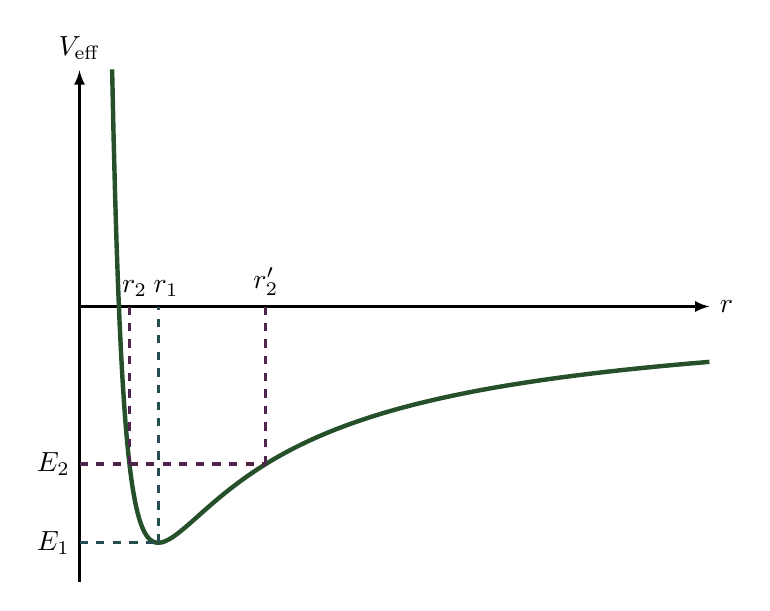
\begin{tikzpicture}
            \draw[->, thick] (0, -3.5) -- (0, 3) node[above] {\(V_\eff\)};
            \draw[->, thick] (0, 0) -- (8, 0) node[right] {\(r\)};
            \draw[domain=0.414:8, highlight, ultra thick, samples=400] plot (\x, {3*(\x^-2 - 2*\x^-1)});
            \draw[complementaryteal, dashed, very thick] (0, -3) -- (1, -3);
            \draw[complementaryteal, dashed, very thick] (1, -3) -- (1, 0);
            \node[above] at (1.1, 0) {\(r_1\)};
            \node[left] at (0, -3) {\(E_1\)};
            \draw[complementarypurple, dashed, very thick] (0, -2) -- (2.366, -2);
            \node[left] at (0, -2) {\(E_2\)};
            \draw[complementarypurple, dashed, very thick] (0.634, -2) -- (0.634, 0);
            \node[above] at (0.7, 0) {\(r_2\)};
            \draw[complementarypurple, dashed, very thick, text=black] (2.366, -2) -- (2.366, 0) node[above] {\(r_2'\)};
        \end{tikzpicture}
        \caption{The effective potential, \(V_{\eff}\).}
        \label{fig:effective central potential}
    \end{figure}
    
    Now consider the particular case where \(E = E_1 = \min V_{\eff}(r)\).
    In this case the particle is constrained to have \(r = r_1\) where \(r_1\) is the value that minimises \(V_\eff\).
    This corresponds to a stable circular orbit.
    
    If instead \(E = E_2 > E_1\) then the particle will be able to move in the radial direction.
    If \(E < 0\) then the particle will be constrained between two values \(r_2\) and \(r_2'\) which are such that \(V_{\eff}(r_2) = V_{\eff}(r_2') = E_2\).
    At \(r_2\) and \(r_2'\) we must have \(\dot{r} = 0\) since these are turning points.
    
    We can treat both of these two cases a bit more formally by considering the effective equation of motion for motion in the radial direction.
    We can find this using energy conservation since this implies \(\dot{E} = 0\):
    \begin{align}
        \diff{E}{t} &= \diff*{\left( \frac{1}{2}m\dot{r}^2 + V_{\eff}(r) \right)}{t}\\
        &= m\dot{r}\ddot{r} + \diff{V_{\eff}}{r}\dot{r}.
    \end{align}
    Since this holds for all \(\dot{r}\) we must have
    \begin{equation}
        m\ddot{r} = -\diff{V_{\eff}}{r}.\label{eqn:EoM central potential}
    \end{equation}
    
    \subsection{Circular Orbit}
    Suppose the particle is in a circular orbit with some fixed radius, \(r = r_1\).
    Then \(\dot{r} = 0\).
    This requires that \(E = V_{\eff}(r_1) = E_1\).
    Therefore a stable circular orbit is possible where the effective potential is a minima or maxima.
    
    Alternatively we know that \(r\) is constant so \(\dot{r}\) and \(\ddot{r}\) are zero meaning that \cref{eqn:EoM central potential} gives
    \begin{equation}
        0=\diff{V_{\eff}}{r}[r=r_1].
    \end{equation}
    
    \subsection{Perturbed Circular Orbit}
    Suppose we have a circular orbit of radius \(r_1\), and we perturb it by moving the particle a small amount, \(\varepsilon\), outwards.
    The radial velocity of the particle is simply
    \begin{equation}
        \dot{r} = \diff*{(r_1 + \varepsilon)}{t} = \dot{\varepsilon}
    \end{equation}

    For small \(\varepsilon\) we can Taylor expand the effective potential about \(r = r_1\):
    \begin{align}
        V_\eff(r) &= V_{\eff}(r_1 + \varepsilon)\\
        &= V_\eff(r_1) + \varepsilon\diff{V_{\eff}}{r}[r=r_1] + \frac{\varepsilon^2}{2}\diff[2]{V_{\eff}}{r}[r=r_1] + \order(\varepsilon^3)\\
        &= V_\eff(r_1) + \frac{k}{2}\varepsilon^2 + \order(\varepsilon^3).
    \end{align}
    Here we have used the fact that \(V_\eff'(r_1) = 0\) as this \(r_1\) is the location of the minimum.
    \(V_\eff(r_1)\) is just a constant and we have defined \(k = V_\eff''(r_1)\).
    Ignoring terms \(\order(\varepsilon^3)\) or smaller and dropping the constant \(V_{\eff}(r_1)\) term we have
    \begin{equation}
        E = \frac{1}{2}m\dot{\varepsilon}^2 + \frac{k}{2}\varepsilon^2.
    \end{equation}
    If \(k > 0\), i.e. \(r_1\) is a local minimum, then this is the energy of a harmonic oscillator of mass \(m\) and spring constant \(k\).
    The small perturbation then leads to the radial position oscillating with angular frequency \(\omega = \sqrt{k/m}\) about \(r_1\).
    
    If \(k < 0\), i.e. \(r_1\) is a local maximum, then the circular orbit is unstable and the perturbation will cause it to turn into some other kind of orbit.
    
    If \(k = 0\) then we can't ignore the \(\order(\varepsilon^3)\) terms in the Taylor expansion.
    
    \subsection{Zones of Motion}
    We showed in the previous example that motion was restricted to the zone \(r_{\mathrm{min}} \le r \le r_{\mathrm{max}}\) where the boundaries are the roots of \(V_{\eff}(r) = E\).
    
    This can be generalised by noticing that \cref{eqn:central potential radial velocity} is of the form
    \begin{equation}
        \dot{r} = \pm \sqrt{g(r)},
    \end{equation}
    in this case \(g(r) = 2(E - V_{\eff}(r))/m\).
    Since \(\dot{r}\) is strictly real this requires \(g(r)\) be positive.
    Therefore whatever happens (barring things like quantum tunnelling) the motion is restricted to th zone \(r_{\mathrm{min}} \le r \le r_{\mathrm{max}}\) where the boundaries are roots of \(g(r) = 0\) at which \(g\) crosses the axis.
    There may be multiple regions in which motion can occur but the system will not be able to move between them unaided.
    
    Analysing various zones of motion can be a powerful tool that allows us to find information about a system without needing to solve for the full trajectory, which is often a difficult task.
    To show that a coordinate is restricted to some zone first look for equations of the form \(\dot{r} = \pm\sqrt{g(r)}\).
   
    \chapter{Dynamics of a Particle System}
    In this section we will consider a system of \(N\) particles, each labelled by some index \(a = 1, \dotsc, N\).
    We suppose that the \(a\)th particle has constant mass \(m_a\) and its position is \(\vv{r_a}\).
    
    We start with Newton's second law for an individual particle:
    \begin{equation}
        m_a\ddot{\vv{r}}_{\vv{a}} = \vv{F_a}.
    \end{equation}
    The force \(\vv{F_a}\) is due to two different sources.
    First there is the external force, \(\vv{F_a^{\ext}}\), which may be, for example, gravity.
    There is also then the force due to interactions with all of the other particles, perhaps due to an electromagnetic interaction.
    We use \(\vv{F_{ab}}\) to denote the force on particle \(a\) due to particle \(b\).
    The total internal force on \(a\) is then given by summing over this interaction for all particles distinct from \(a\).
    The net force on the particle is then
    \begin{equation}
        \vv{F_a} = \vv{F_a^{\ext}} + \sum_{b \ne a} \vv{F_{ab}}.
    \end{equation}
    
    \section{Centre of Mass Motion}
    Summing Newton's law over all particles we get
    \begin{equation}
        \sum_{a} m_a\ddot{\vv{r}}_{\vv{a}} = \sum_a\vv{F_a} = \sum_a \vv{F_a^{\ext}} + \sum_a \sum_{b\ne a} \vv{F_{ab}}.
    \end{equation}
    Focussing on this last term with a double sum we see that it is possible to write it as a single sum over pairs of particles,
    \begin{equation}
        \sum_{a}\sum_{b\ne a} \vv{F_{ab}} = \sum_{\text{pairs}} (\vv{F_{ab}} + \vv{F_{ba}}).
    \end{equation}
    To see this consider the explicit example of three particles:
    \begin{align}
        \sum_{a=1}^{3}\sum_{\substack{b\in\{1, 2, 3\}\\b\ne a}} \vv{F_{ab}} &= \vv{F_{12}} + \vv{F_{13}} + \vv{F_{21}} + \vv{F_{23}} + \vv{F_{31}} + \vv{F_{32}}\\
        &= (\vv{F_{12} + \vv{F_{21}}}) + (\vv{F_{13}} + \vv{F_{31}}) + (\vv{F_{23}} + \vv{F_{32}}).
    \end{align}
    
    It follows, assuming the weak form of Newton's third law, that \(\vv{F_{ba}} = -\vv{F_{ab}}\) and hence
    \begin{equation}
        \sum_{a}\sum_{b\ne a} \vv{F_{ab}} = \sum_{\text{pairs}}(\vv{F_{ab}} + \vv{F_{ba}}) = \sum_{\text{pairs}} (\vv{F_{ab}} - \vv{F_{ab}}) = \vv{0}.
    \end{equation}
    So, all internal forces cancel pairwise.
    Hence
    \begin{equation}
        \sum_a m_a\ddot{\vv{r}}_{\vv{a}} = \sum_a \vv{F_{a^{\ext}}} \eqqcolon \vv{F^{\ext}}
    \end{equation}
    where we have defined \(\vv{F^{\ext}}\) to be the net external force on the system.
    Defining the total mass
    \begin{equation}
        M \coloneqq \sum_a m_a
    \end{equation}
    we can define the \defineindex{centre of mass} to be
    \begin{equation}
        \vv{R} \coloneqq \frac{1}{M}\sum_a m_a\vv{r_a}.
    \end{equation}
    We can think of it as the average position of the particles weighted by their masses.
    
    Differentiating this definition twice leads to
    \begin{equation}
        M\ddot{\vv{R}} = \vv{F^{\ext}}.
    \end{equation}
    We can also define the total linear momentum
    \begin{equation}
        \vv{P} \coloneqq \sum_a \vv{p_a} = \sum_a m_a \dot{\vv{r}}_{\vv{a}} = M\dot{\vv{R}}.
    \end{equation}
    From this we see that
    \begin{equation}
        \dot{\vv{P}} = \vv{F^{\ext}}.
    \end{equation}
    This means that the centre of mass acts as a point particle obeying Newton's second law in the presence of the net external force.
    We use this implicitly whenever we do dynamics since all bodies are really made up of many particles but we almost exclusively consider rigid bodies to be point particles at their centre of mass.
    
    \section{Angular Motion}
    Starting with Newton's second law, this time in the form \(\dot{\vv{p_a}} = \vv{F_a}\), we can take the cross product with \(\vv{r_a}\) and sum over all particles giving
    \begin{equation}\label{eqn:angular motion system of particles}
        \sum_a \vv{r_a}\times\dot{\vv{p}}_{\vv{a}} = \sum_a \vv{r_a}\times\vv{F_a}.
    \end{equation}

    Using the trick of recognising the left hand side as half of a product rule we have
    \begin{equation}
        \vv{r_a}\times\dot{\vv{p}}_{\vv{a}} = \diff*{(\vv{r_a}\times\vv{p_a})}{t} - \dot{\vv{r}}_{\vv{a}}\times\vv{p_a} = \diff{\vv{L_a}}{t} - \dot{\vv{r_a}} \times \vv{p_a}.
    \end{equation}
    The second term is zero since \(\vv{p_a} = m_a\dot{\vv{r}}_{\vv{a}}\) and hence we have
    \begin{equation}
        \dot{\vv{L}} \coloneqq \sum_a \vv{L_a} = \sum_a \vv{r_a}\times\dot{\vv{p}}_{\vv{a}}.
    \end{equation}
    
    Returning to the right hand side of \cref{eqn:angular motion system of particles} we have
    \begin{equation}
        \sum_a \vv{r_a}\times\vv{F_a} = \sum_a \vv{r_a} \times \vv{F_a^{\ext}} + \sum_{a}\sum_{b\ne a}\vv{r_a}\times\vv{F_{ab}}.
    \end{equation}
    Using the weak form of Newton's third law we can again move to a sum over pairs of particles and the last term becomes
    \begin{equation}
        \sum_{a}\sum_{b\ne a} \vv{r_a}\times \vv{F_{ab}} = \sum_{\text{pairs}} (\vv{r_a}\times \vv{F_{ab}} + \vv{r_b}\times\vv{F_{ba}}) = \sum_{\text{pairs}} (\vv{r_a} - \vv{r_b})\times\vv{F_{ab}}.
    \end{equation}
    Assuming the strong form of Newton's third law this is \(\vv{0}\) since \(\vv{r_a} - \vv{r_b}\) and \(\vv{F_{ab}}\) both point along the line between the two particles.
    In this case the total angular momentum obeys
    \begin{equation}
        \dot{\vv{L}} = \sum_a \vv{r_a}\times\vv{F_a^{\ext}} = \sum_a \vv{G_a^{\ext}} \eqqcolon \vv{G^{\ext}}
    \end{equation}
    where \(\vv{G_a^{\ext}}\) is the external torque on the \(a\)th particle and \(\vv{G^{\ext}}\) is the net external torque.
    That is, these torques are due to external forces.
    
    It should be noted that both \(\vv{L}\) and \(\vv{G}\) depend on our choice of origin.
    
    \section{Energy}
    For a single particle we have
    \begin{equation}
        \vv{F}\cdot\dl{\vv{r}} = \dd{\left( \frac{1}{2}mv^2 \right)} = \dd{T}.
    \end{equation}
    Here \(T\) is the kinetic energy.
    For \(N\) particles we then have
    \begin{align}
        \dd{T} &= \sum_a \dd{T_a}\\
        &= \sum_a \vv{F_a}\cdot\dl{\vv{r_a}}\\
        &= \sum_a \vv{F_a^{\ext}}\cdot\dl{\vv{r_a}} + \sum_{\text{pairs}} \vv{F_{ab}}\cdot(\dl{\vv{r_a}} - \dl{\vv{r_b}}).
    \end{align}
    Again, we have converted a sum over \(a\) and \(b \ne a\) into a sum over pairs of particles.
    
    If the external force is conservative then there is a potential function of the form \(V(\vv{r_1}, \dotsc, \vv{r_N})\) such that
    \begin{equation}
        \vv{F_a^{\ext}} = -\grad[a] V
    \end{equation}
    where \(\grad[a]\) is the gradient with respect to \(\vv{r_a}\).
    It then follows that
    \begin{equation}
        \sum_a\vv{F_a^{\ext}}\cdot\dl{\vv{r_a}} = -\dl{V}.
    \end{equation}
    
    If the internal forces are conservative then there is a potential function of the form \(U(\vv{r_1}, \dotsc, \vv{r_N})\) such that
    \begin{equation}
        \vv{F_{ab}} = -\grad[a] U.
    \end{equation}
    The weak form of Newton's third law then gives us
    \begin{equation}
        \vv{F_{ba}} = -\grad[b]U = \grad[a]U.
    \end{equation}
    The only way that this can hold is if the potential depends only on the vector \(\vv{r_{ab}} = \vv{r_a} - \vv{r_b}\), which connects the two particles.
    
    Defining \(\grad[ab]\) as the gradient with respect to \(\vv{r_{ab}}\) this becomes
    \begin{equation}
        \vv{F_{ab}} = -\grad[ab]U = \grad[ba] U.
    \end{equation}
    We then have
    \begin{equation}
        \sum_{\text{pairs}} \vv{F_{ab}} \cdot(\dl{\vv{r_a}} - \dl{\vv{r_b}}) = -\sum_{\text{pairs}}\grad[ab]U\cdot\dl{\vv{r_{ab}}} = -\dd{U}.
    \end{equation}
    
    Combining the results of this section we have
    \begin{equation}
        \dd{T} = -\dd{V} - \dd{U} \implies \dd{T} + \dd{V} + \dd{U} = 0.
    \end{equation}
    What this means is that the total change in energy, which is the change in kinetic energy, and external and internal potential energies, is zero.
    So, assuming conservative forces and the weak form of Newton's third law energy is conserved.
    
    \chapter{Transforming Between Frames}
    \section{Galilean Transformations}
    A \defineindex{Galilean transformation} is a non-relativistic transformation between inertial frames.
    Suppose that frame \(S'\) moves at constant velocity, \(\vv{V}\), with respect to the frame \(S\) and that the origin of \(S'\) is related to the origin of \(S\) by \(O' = O + \vv{b}\) at time \(t = 0\).
    Note that it is common to assume \(\vv{b} = \vv{0}\) and the origins coincide at \(t = 0\), and also that the axes of the two frames are parallel and motion is in the \(x\) direction.
    This is called the standard configuration but we will deal with this slightly more general case.
    
    Let \(\vv{r}\) be a position vector in frame \(S\), and let \(\vv{r'}\) be the same position in frame \(S'\).
    Notice that these two vectors refer to the same point in different frames.
    In the language of coordinate transforms this means that we transform between frames with passive transformations.
    It follows from the geometry of our set up that at time \(t = 0\) \(\vv{r} = \vv{r'} + \vv{b}\).
    At some later time \(t\) we then have 
    \begin{equation}
        \vv{r} = \vv{r'} + \vv{b} + t\vv{V}.
    \end{equation}
    This is the Galilean transformation for positions.
    
    Differentiating this we get
    \begin{equation}
        \vv{v} = \vv{v'} + \vv{V}
    \end{equation}
    where \(\vv{v}\) and \(\vv{v'}\) are the velocity of the point in frames \(S\) and \(S'\), respectively.
    This is the Galilean transformation for velocities.
    
    Suppose now that this point is the position of one of our particles from the previous chapter.
    Multiplying the velocity transform by the mass, \(m_a\), we have
    \begin{equation}
        \vv{p_a} = \vv{p_a'} + m_a\vv{V}
    \end{equation}
    where \(\vv{p_a}\) and \(\vv{p_a'}\) are the momentum of the particle as measured in frames \(S\) and \(S'\) respectively.
    Differentiating this we have
    \begin{equation}
        \dot{\vv{p}}_{\vv{a}} = \dot{\vv{p}}\vv{_a'} = \vv{F_a},
    \end{equation}
    which shows us that force is Galilean invariant.
    
    From this the transformation for the properties of the entire system follow.
    In particular
    \begin{equation}
        \vv{P} = \vv{P'} + M\vv{V}, \qqand \dot{\vv{P}} = \dot{\vv{P}}\vv{'} = \vv{F^{\ext}}.
    \end{equation}
    This means that Newton's laws are unaffected by a Galilean transformation and are the same in any inertial frame.
    That is they are Galilean invariant.
    
    \subsection{Centre of Momentum Frame}
    \begin{dfn}{Centre of Momentum Frame}{}
        The \defineindex{centre of momentum frame} (CoM frame)\glossary[acronym]{CoM}{centre of momentum} is defined as the \emph{inertial} frame chosen \emph{instantaneously} such that 
        \begin{equation}
            \vv{P'} = \sum_{a}\vv{p_a'} = \sum_{a} m_a\dot{\vv{r}}\vv{_a'} = \vv{0}.
        \end{equation}
        That is, the total momentum is instantaneously zero.
    \end{dfn}
    
    The centre of mass frame is only defined at a single time, this is so that it is an inertial frame.
    
    We often choose the centre of mass to be the origin of the centre of momentum frame, that is \(\vv{R'} = \vv{0}\).
    Taking the position of each particle and multiplying by its mass before summing over all particles gives us
    \begin{equation}
        \sum_a m_a\vv{r_a} = \sum_a m_a\vv{r_a'} + \sum_a m_at\vv{V} + \sum_a m_a\vv{b}
    \end{equation}
    or in terms of global properties
    \begin{equation}
        M\vv{R} = M\vv{R'} + Mt\vv{V} + M\vv{b}.
    \end{equation}
    Taking the origin as the centre of mass we find
    \begin{equation}
        \vv{b} = \vv{R} - t\vv{V}.
    \end{equation}
    
    A related concept is the \defineindex{centre of mass frame} which is the frame with its origin at the centre of mass at all times.
    This frame will be non-inertial if there is a net external force.
    
    \subsection{Intrinsic Angular Momentum}
    The angular momentum of a single particle at time \(t = 0\) is given by
    \begin{equation}
        \vv{L_a} = \vv{r_a} \times \vv{p_a} = (\vv{r_a'} + \vv{b})\times \vv{p_a'} = \vv{r_a'}\times\vv{p_a'} + \vv{b}\times\vv{p_a'} = \vv{L_a'} + \vv{b}\times\vv{p_a'}.
    \end{equation}
    The total angular momentum at some time \(t\) is then
    \begin{align}
        \vv{L} &= \sum_a \vv{r_a} \times \vv{p_a}\\
        &= \sum_a (\vv{r'_a} + t\vv{V} + \vv{b})\times (\vv{p_a'} + m_a\vv{V})\\
        &= \vv{L'} + M\vv{R'} \times \vv{V} + (t\vv{V} + \vv{b}) \times \vv{P'} + M(t\vv{V} + \vv{b})\times\vv{V}.
    \end{align}
    Define \(\vv{J} = \vv{L'}\) to be the \defineindex{intrinsic angular momentum}, that is the angular momentum due to the \emph{internal} motion of the particles in the centre of momentum frame.
    In this frame we also have \(\vv{P'} = \vv{0}\), \(\vv{R'} = \vv{0}\), \(t\vv{V} + \vv{b} = \vv{R}\), and \(\vv{P} = M\vv{V}\) and so we get
    \begin{equation}
        \vv{L} = \vv{J} + \vv{R} \times \vv{P}.
    \end{equation}
    
    What this shows is that the angular momentum in some frame, \(S\), is the intrinsic angular momentum of the particles, plus the angular momentum due to the motion of the centre of mass.
    From this we also see that \(\vv{L}\) depends on the choice of origin (unless \(\vv{P} = \vv{0}\).
    
    Performing a similar calculation for the external torque we find
    \begin{equation}
        \vv{G^{\ext}} = (\vv{G^{\ext}})' + \vv{b}\times\vv{F^{\ext}}.
    \end{equation}
    Notice that the extra term from moving the origin \emph{doesn't} vanish in the torque expression and therefore we must always specify the origin of the centre of momentum frame when we discuss torque.
    
    \subsection{Kinetic Energy Transformation}
    In frame \(S\) the kinetic energy is
    \begin{align}
        T &= \sum_a \frac{1}{2}m_av_a^2\\
        &= \sum_a \frac{1}{2}m_a(\vv{v_a}' + \vv{V})\cdot (\vv{v_a'} + \vv{V})\\
        &= \sum_a\frac{1}{2}m_a(v_a')^2 + \sum_a m_a\vv{v_a'}\cdot\vv{V} + \sum_a \frac{1}{2}m_aV^2\\
        &= T' + \sum_a m_a\vv{v_a'}\cdot\vv{V} + \frac{1}{2}MV^2.
    \end{align}
    Taking \(S'\) to be the centre of momentum frame this central term vanishes is \(\vv{P'}\cdot\vv{V} = 0\), and we have
    \begin{equation}
        T = T' + \frac{1}{2}MV^2
    \end{equation}
    So, the kinetic energy in some frame, \(S\), is the kinetic energy in the centre of momentum frame plus a contribution due to motion of the centre of mass.
    
    \section{Rotating Frame}
    Occasionally we will have need to work in a rotating frame.
    Note that rotating frames are necessarily non-inertial so the work from earlier on in this chapter \emph{does not apply}.
    We will consider only the simplest example of a frame, \(R\), rotating with respect to some inertial frame, \(S\), with constant angular velocity, \(\vv{\omega}\).
    Further we set up the axes and time such that at time \(t = 0\) the axes and origins of \(R\) and \(S\) are coincident.
    We will use the notation \([f]_X\) to denote the quantity \(f\) as measured in frame \(X\).
    
    Consider a position vector in \(R\), \([\vv{r}]_{R}\).
    Quantities without subscripts are taken to have been measured at time \(t = 0\) and hence are the same in both frames.
    If this is stationary in \(R\) then from \(S\) it is seen as rotating with velocity
    \begin{equation}
        [\vv{v}]_S = \vv{\omega} \times \vv{r}
    \end{equation}
    where \(\vv{r} = [\vv{r}(t = 0)]_R = [\vv{r}(t = 0)]_S\) is the position at time \(t = 0\).
    If the position instead has some nonzero velocity in \(R\) then the velocity in \(S\) is
    \begin{equation}
        [\dot{\vv{r}}]_S = [\dot{\vv{r}}]_R + \vv{\omega}\times\vv{r}.
    \end{equation}
    
    Consider a general vector, \(\vv{A}\).
    In a short time, \(\dl{t}\), in the rotating frame
    \begin{equation}
        [\vv{A}]_R \to [\vv{A}]_R + [\dl{\vv{A}}]_R,
    \end{equation}
    and in the stationary frame
    \begin{equation}
        [\vv{A}]_S \to ([\vv{A}]_R + [\dl{\vv{A}}]_R) + \vv{\omega}\times\vv{A}\dl{t}.
    \end{equation}
    Together these imply that
    \begin{equation}
        [\dl{\vv{A}}]_S = \dl{\vv{A}} + \vv{\omega}\times\vv{A}\dl{t}.
    \end{equation}
    Or, equivalently
    \begin{equation}
        [\dot{\vv{A}}]_S = [\dot{\vv{A}}]_R + \vv{\omega}\times\vv{A}.
    \end{equation}
    Setting \(\vv{A} = \vv{r}\) we recover the equation for velocity transformations in a rotating frame.
    
    Now consider the case of \(\vv{A} = m[\dot{\vv{r}}]_S\).
    We have
    \begin{align}
        m\left[ \diff*{[\dot{\vv{r}}]_S}{t} \right]_S = m\left[ \diff*{[\dot{\vv{r}}]_S}{t} \right]_S.
    \end{align}
    Hence
    \begin{equation}
        m[\ddot{\vv{r}}]_S = m\left[ \diff{}{t}([\dot{\vv{r}}]_R + \vv{\omega}\times\vv{r}) \right]_R + m\vv{\omega} \times [[\dot{\vv{r}}]_R + \vv{\omega}\times\vv{r}]_S.
    \end{equation}
    The left hand side is simply the mass times the acceleration in the inertial frame, \(S\), and hence we can apply Newton's second law and write this term as \(\vv{F}\), the force on the particle.
    We can expand the right hand side and we get
    \begin{equation}
        \vv{F} = m[\ddot{\vv{r}}]_R + m\vv{\omega}\times[\dot{\vv{r}}]_R + m\vv{\omega}\times\vv{\omega}\times[\dot{\vv{r}}]_R + m\vv{\omega}\times(\vv{\omega}\times\vv{r}).
    \end{equation}
    
    Rearranging this we have
    \begin{equation}
        m[\ddot{\vv{r}}]_R = \vv{F} - m\vv{\omega}\times(\vv{\omega}\times\vv{r}) - 2m\vv{\omega}\times[\dot{\vv{r}}]_R
    \end{equation}
    which is equivalent to
    \begin{equation}
        m\vv{a} = \vv{F} - m\vv{\omega}\times(\vv{\omega} \times \vv{r}) - 2m\vv{\omega}\times\vv{v}
    \end{equation}
    where \(\vv{v}\) and \(\vv{a}\) are the velocity and acceleration in the rotating frame.
    
    This is similar in form to Newton's second law and so we identify the two extra terms as \define{fictitious forces}\index{fictitious force}.
    The first is the \defineindex{centrifugal force} and the second the \defineindex{Coriolis force}.
    While these aren't real forces, they arise due to an attempt to treat the non-inertial rotating frame as inertial, they do have observable effects.
    The centrifugal force always acts to cause objects to fly outwards in the rotating frame.
    The Coriolis force acts to cause objects moving in a plane perpendicular to the axis of rotation to be deflected at right angles.
    
    \chapter{Degrees of Freedom and Constraints}
    \section{Degrees of Freedom}
    \begin{dfn}{Degrees of Freedom}{}
        The \define{degrees of freedom}\index{degree of freedom} of a system are a set of variables the values of which are precisely enough to specify the state of the system.
    \end{dfn}
    
    \begin{exm}{Single Particle}{}
        A single particle has three degrees of freedom.
        These correspond to its location.
        There are several equally valid choices of degrees of freedom.
        We could use the three Cartesian coordinates, cylindrical coordinates, spherical coordinates, or many more.
    \end{exm}
    
    The degrees of freedom aren't always as simple as the coordinates of the particles.
    
    \begin{exm}{Pendulum}{}
        A simple pendulum has only one degree of freedom, which we most commonly take to be the angle to the vertical.
        We see from this that constraints, such as being on the end of a rod of fixed length that can only move in a plane, can reduce the number of degrees of freedom.
    \end{exm}
    
    \begin{exm}{Rigid Body}{}
        A \defineindex{rigid body} is a collection of particles fixed such that the particles positions relative to each other are fixed.
        Despite being made of arbitrarily many particles a rigid body has only six degrees of freedom.
        We need to specify location and orientation, this then fixes the position of all particles.
        Most commonly we do this by defining the centre of mass, which takes three degrees of freedom, and the orientation, which can be elegantly done with three Euler angles.
    \end{exm}
    
    The example of a rigid body shows how we can greatly reduce the number of variables to deal with by considering degrees of freedom instead of the coordinates of every particle.
    
    \section{Constraint Forces}
    We have already seen one constraint in our examples above, the pendulum was constrained to motion in a plane that kept it a fixed distance from the point at which it is connected.
    Another example of a constraint may be a particle on the floor, or constrained to move within a box.
    
    Consider some particle, \(a\), with position vector \(\vv{r_a}\), moving subject to some constraint.
    The motion is constrained by a constraint force, \(\vv{F_{\constraint}}\).
    This force acts at right angles to the motion and hence do no work for an instantaneous displacement since \(\vv{F_{\constraint}} \cdot \delta\vv{r} = 0\) for some small displacement, \(\delta\vv{r}\), we will make this more rigorous shortly.
    An example here might be a ball constrained to role down a tube.
    The walls of the tube exert a normal force on the ball only when it is in contact.
    When the ball is in contact with the wall it can only move parallel to the wall and hence perpendicular to the force.
    
    \subsection{Holonomic Constraints}
    \begin{dfn}{Holonomic Constraint}{}
        A holonomic constraint is one which can be written as
        \begin{equation}
            f(\vv{r_1}, \vv{r_2}, \dotsc, \vv{r_N}, t) = 0.
        \end{equation}
        Here \(f\) is an algebraic function of the coordinates and time.
        Specifically this is \emph{not} a differential equation or an inequality.
    \end{dfn}
    
    An example of a holonomic constraint might be a particle on the floor.
    This is equivalent to the constraint that \(z = 0\), where we choose the origin to be on the floor and the \(z\)-axis to be vertical.
    Another example is two particles constrained to be a fixed distance, \(\rho\), apart, since we can write this as \(\abs{\vv{r_a} - \vv{r_b}} = \rho\).
    
    Holonomic constraints can include an explicit time dependence, for example a particle on the floor of a lift is constrained to \(z = vt\) where \(v\) is the speed of the lift which started at \(z = 0\) at time \(t = 0\).
    
    \begin{exm}{Rolling Cylinder}{}
        Consider a cylinder of radius \(a\) rolling down an inclined plane.
        We can set up coordinates such that \(x'\) points down the plane and \(y'\) is normal to the plane.
        In general there are three degrees of freedom.
        The position of the centre of the cylinder, \((x', y')\), and the angle through which it is rotated, \(\vartheta\).
        
        If we impose \defineindex{rolling conditions}, that is that the sphere doesn't bounce, so \(y' = a\), and doesn't slide, so \(x' = a\vartheta + C\) for some constant offset \(C\).
        This gives us two holonomic constraints.
        Notice that the number of degrees of freedom is reduced to 1.
        We can specify either \(x'\) or \(\vartheta\), and are free to choose which, as the other degrees of freedom will then be fixed.
    \end{exm}
    
    \begin{figure}
        \tikzsetnextfilename{rolling-cylinder}
        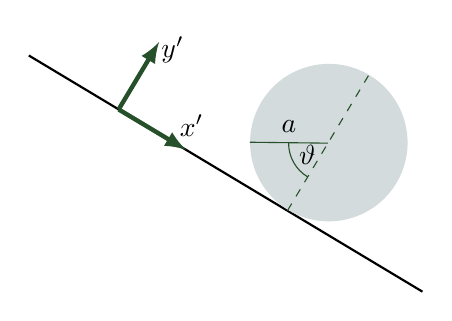
\begin{tikzpicture}
            \draw[thick] (0, 3) -- (5, 0);
            \fill[complementaryteal!20, rotate around={-31.3:(5, 0)}] (3, 1) circle [radius = 1];
            \begin{scope}[rotate around={-30.96:(5, 0)}]
                \draw[highlight, ultra thick, ->] (0.5, 0) -- (1.5, 0);
                \draw[highlight, ultra thick, ->] (0.5, 0) -- (0.5, 1);
                \node at (1.4, 0.3) {\(x'\)};
                \node at (0.7, 1) {\(y'\)};
                \draw[highlight, dashed] (3, 0) -- (3, 2);
                \draw[highlight, text=black] (3, 1) -- (2.144, 0.5) node[midway, above] {\(a\)};
                \path (2.144, 0.5) coordinate (A) -- (3, 1) coordinate (B) -- (3, 0) coordinate (C) pic [draw, "\(\vartheta\)", angle radius=0.5cm, highlight, text=black] {angle=A--B--C};
            \end{scope}
        \end{tikzpicture}
        \caption{A cylinder of radius \(a\) rolls down an inclined plane. There are initially three degrees of freedom, \(x'\), \(y'\), and \(\vartheta\), which is reduced to one degree of freedom by imposing rolling conditions.}
    \end{figure}
    
    In general each holonomic constraint decreases the number of degrees of freedom by one.
    
    \subsection{Nonholonomic Constraints}
    Unsurprisingly \defineindex{nonholonomic constraints} are those which aren't holonomic, that is they can't be written as a simple algebraic equation of the coordinates and time.
    Most often they come in the form of inequalities or differential equations.
    
    \begin{exm}{Inequality Constraint}{}
        A particle is constrained to move in a rectangular box of width \(a\) and height \(b\).
        This is a nonholonomic constraint since the constraint is equivalent to
        \begin{equation}
            0 \le x \le a, \qqand 0 \le y \le b.
        \end{equation}
        Notice that this is a two dimensional problem and as such there are initially two degrees of freedom.
        After imposing the constraint there are still two degrees of freedom.
    \end{exm}
    
    \begin{exm}{Differential Constraint}{}
        Consider a hoop of radius \(a\) rolling along a plane.
        This has five degrees of freedom, the location of the centre of the hoop, \((x, y, z)\), the angle through which the hoop is rotated, \(\varphi\), and the direction in which the hoop roles, for example the angle of this line to the \(x\)-axis, \(\vartheta\).
        
        Unlike the one-dimensional case introducing rolling constraints only reduces the number of degrees of freedom by 1.
        We have now fixed \(z = a\).
        Intuitively this is because the extra freedom of an second dimension allows us to return to the same spot with a different angle of rotation by rolling in a circle with a non-integer ratio of its radius to \(a\).
        Mathematically this is because the constraints we now have are that a small change in the angle, \(\dl{\varphi}\), corresponds to a change \(\dl{r} = a\dl{\varphi}\), where \(\dl{r}\) is a small displacement along the direction of rolling.
        Decomposing into \(x\) and \(y\) changes we have that \(\dl{x} = a\cos\vartheta\dl{\varphi}\) and \(\dl{y} = a\sin\vartheta\dl{\varphi}\).
        This gives the nonholonomic constraints
        \begin{equation}
            \dot{x} = a\dot{\varphi}\cos\vartheta, \qqand \dot{y} = a\dot{\varphi}\sin\vartheta.
        \end{equation}
        These constraints \emph{cannot} be integrated to get holonomic constraints as \(\vartheta\) is a function of time.
        
        Note that we can write the rolling constraint for the one-dimensional example in a differential equation form as \(\dot{x}' = a\dot{\vartheta}\), but this can immediately be integrated to give \(x' = a\vartheta + C\) for some constant \(C\) and so this is still a holonomic constraint.
    \end{exm}

    \begin{figure}
        \tikzsetnextfilename{rolling-in-plane}
        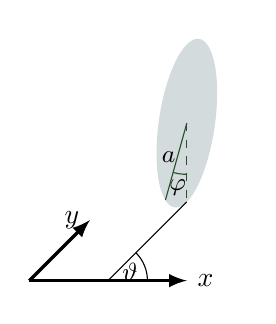
\begin{tikzpicture}
            \draw[very thick, ->] (0, 0, 2) -- (0, 0, 0) node [left] {\(y\)};
            \draw[very thick, ->] (0, 0, 2) -- (2, 0, 2) node [right] {\(x\)};
            \fill[very thick, complementaryteal!20, canvas is yz plane at x=2] (2, 2) circle [radius = 1];
            \draw[highlight, dashed, canvas is yz plane at x=2] (2, 2) -- (1, 2);
            \draw[highlight, canvas is yz plane at x=2, text=black] (2, 2) -- (2 - 1.41/2, 2 + 1.41/2);
            \node at (2, 1.8, 2.6) {{\small\(a\)}};
            \path[canvas is yz plane at x=2] (1, 2) coordinate (C) -- (2, 2) coordinate (B) -- (2 - 1.41/2, 2 + 1.41/2) coordinate (A);
            \draw pic [draw, highlight, angle radius=0.65cm] {angle};
            \node at (2, 1.3, 2.3) {{\small\(\varphi\)}};
            \draw (2, 1, 2) -- (1, 0, 2);
            \path[canvas is xz plane at y=0] (2, 2) coordinate (A) -- (1, 2) coordinate (B) -- (2, 0) pic [draw, "{\small\(\vartheta\)}"] {angle};
        \end{tikzpicture}
        \caption{A hoop rolling in the plane has five initial degrees of freedom, \(x\), \(y\), \(z\), \(\varphi\), and \(\vartheta\). Introducing rolling constraints reduces this to four degrees of freedom by fixing \(z = a\).}
    \end{figure}
    
    \chapter{Generalised Quantities}
    Often our degrees of freedom are coordinates, in particular Cartesian coordinates.
    However, this isn't always the case, for example the angle of rotation is not a Cartesian coordinate.
    Our goal in this chapter is to come up with a generalisation for several classical quantities, specifically coordinates, velocities, and force, which keep the key properties but allow us to be more general.
    We will also see generalised momentum in later chapters.
    
    \begin{ntn}{}{}
        Given some indexed quantity, \(x_i\), with \(i = 1, \dotsc, N\) we will use \(\{x\}\) as shorthand for \(x_1, x_2, \dotsc, x_N\).
    \end{ntn}

    \section{Generalised Coordinates}
    Consider some system of particles in three dimensions.
    Particle \(a\) has three coordinates, \(\vv{r_a} = (x_a, y_a, z_a)\).
    Given a list of all of the particles coordinates,
    \begin{equation}
        x_1, y_1, z_1, x_2, y_2, z_2, \dotsc, x_N, y_N, z_N,
    \end{equation}
    we have \(3N\) coordinates, for which we use the shorthand \(x_i\) with \(i = 1, \dotsc, 3N\).
    
    In the presence of holonomic constraints these \(x_i\) are not all independent.
    If we have \(M\) holonomic constraints then there are \(3N - M\) independent variables, \(q_i\), which describe the state of the system at a given time.
    We can view these as functions of the form
    \begin{equation}\label{eqn:q as func of x}
        q_i = q_i(x_1, x_2, \dotsc, x_{3N}, t) = q_i(\{x\}, t), \qquad\text{for } i = 1, \dotsc, 3N - M.
    \end{equation}
    A general aim in this course will be to generate \(3N - M\) second order differential equations in these \(q_i\).
    These are the \define{equations of motion}\index{equation of motion} (EoM)\glossary[acronym]{EoM}{equation of motion}.
    The variables \(\{q\}\) are our \define{generalised coordinates}\index{generalised coordinate}.
    
    We assume that the relation in \cref{eqn:q as func of x} is invertible and so we have
    \begin{equation}
        x_i = x_i(q_1, q_2, \dotsc, q_{3N-M}, t) = x_i(\{q\}, t), \qquad\text{for } i = 1, \dotsc, 3N.
    \end{equation}
    This allows us to recover information about the original system by solving the equations of motion for \(\{q\}\).
    The important point is that \(q_i\) can be individually varied, which we will use to derive the equations of motion, whereas we cannot vary all \(x_i\) without changing at least one other \(x_j\).
    
    \subsection{Generalised Velocities}
    The \define{generalised velocities}\index{generalised velocity} are simply the time derivatives of the generalised coordinates.
    That is, \(\dot{q}_i\), or collectively \(\{\dot{q}\}\).
    
    It should be noted that until we apply the equations of motion we can treat \(\{q\}\) and \(\{\dot{q}\}\) independently as we are considering arbitrary motion of the system.
    This means that we can just treat \(\{\dot{q}\}\) as another set of variables until we start solving the equations of motion.
    
    \section{Generalised Force}
    Consider an infinitesimal change in the coordinates, \(x_i \to x_i + \dl{x_i}\).
    This is a \defineindex{generalised displacement}.
    A simple application of the chain rule gives us
    \begin{equation}
        \dl{x_i} = \sum_j \diffp{x_i}{q_j}\dl{q_j} + \diffp{x_i}{t}\dl{t}.
    \end{equation}
    
    We define a \defineindex{virtual displacement} to be an instantaneous, infinitesimal displacement with no \(\dl{t}\) component.
    To distinguish from a normal displacement we write this as \(\delta x_i\).
    Again applying the chain rule, with the \(\dl{t}\) component vanishing, we have
    \begin{equation}
        \delta x_i = \sum_j \diffp{x_i}{q_j}\dl{q_j}.
    \end{equation}
    
    The work done in a virtual displacement due to forces \(F_i\) in the direction of \(\delta x_i\) is
    \begin{equation}
        \delta W = \sum_i F_i\delta x_i.
    \end{equation}
    We can split the force into a constraint force, and other sources of force, \(F_i^{\other}\).
    Since constraint forces do no work the work done reduces to
    \begin{equation}
        \delta W = \sum_{i} F_{i}^{\other} \delta x_i.
    \end{equation}
    We can write this in terms of \(\{\delta q\}\) using the chain rule:
    \begin{equation}
        \delta W = \sum_j \sum_i F_i^{\other} \diffp{x_i}{q_j}\delta q_j = \sum_j Q_j \delta q_j
    \end{equation}
    where we have defined the \defineindex{generalised force}
    \begin{equation}
        Q_j \coloneqq \sum_{i}F_i^{\other} \diffp{x_i}{q_j}.
    \end{equation}
    
    It should be noted that generalised quantities do not necessarily have the same dimensions as the quantity they generalise.
    For example an angle is dimensionless but may be a valid generalised coordinate, \(q\), where we would expect coordinates to have dimensions of length.
    The work done has units of energy so in this case the generalised force, \(Q\), must have units of energy so that the product \(qQ\) has units of energy.
    
    \begin{exm}{Particle on a Hoop}{exm:particle on a hoop}
        A particle of mass \(m\) slides under gravity around a smooth vertical hoop of radius \(a\).
        Taking the centre of the hoop as the origin in Cartesian coordinates we have two coordinates, \((x, z)\), to describe the position of the particle.
        We also have one holonomic constraint, that \(x^2 + z^2 = a^2\).
        Hence, there is one degree of freedom.
        
        The sensible choice for a generalised coordinate here is an angle.
        For no particular reason we choose the angle to the vertical measuring anticlockwise.
        This quantity, \(\vartheta\), is related to the Cartesian position by
        \begin{equation}
            x = -a\sin\vartheta, \qqand z = a\cos\vartheta.
        \end{equation}
    
        The force on the particle consists of a constraint force from the hoop, and the force due to gravity, \(\vv{F^{\other}} = (0, -mg)\).
        The work done on the particle in a virtual displacement, \(\delta\vartheta\), is
        \begin{align}
            \delta W &= \left[ F_x^{\other} \diffp{x}{\vartheta} + F_z^{\other} \diffp{z}{\vartheta} \right]\delta\vartheta\\
            &= 0 + (-mg)\diffp*{(a\cos\vartheta)}{\vartheta}\delta\vartheta\\
            &= (mga\sin\vartheta)\delta\vartheta.
        \end{align}
        From this we identify the generalised force
        \begin{equation}
            Q_{\vartheta} = mga\sin\vartheta.
        \end{equation}
        
        This has dimensions of energy, so \(\vartheta Q_\vartheta\) has units of energy also.
    \end{exm}
    
    \section{Functions of \texorpdfstring{\(\{q\}\), \(\{\dot{q}\}\), and \(t\)}{\{q\}, \{q-dot\}, and t}}
    We will often deal with functions of \(\{q\}\), \(\{\dot{q}\}\), and \(t\).
    For example the kinetic energy,
    \begin{equation}
        T = \sum_i \frac{1}{2}m_i\dot{x}_i^2.
    \end{equation}
    Since \(x_i = x_i(\{q\}, t)\) in generalised coordinates the kinetic energy can depend explicitly on \(\{q\}\) and \(\{\dot{q}\}\), for example in polar coordinates we saw that the kinetic energy was
    \begin{equation}
        T = \frac{1}{2}m(\dot{r}^2 + r^2\dot{\varphi}^2).
    \end{equation}
    This depends on the generalised coordinate \(r\) and the generalised velocities \(\dot{r}\) and \(\dot{\varphi}\).
    
    For such functions we can write a small increment, \(\dl{f}\), as
    \begin{equation}
        \dl{f} = \sum_j \diffp{f}{q_j} \dl{q_j} + \sum_j \diffp{f}{\dot{q}_j} \dl{\dot{q}_j} + \diffp{f}{t}\dl{t}.
    \end{equation}
    Note that we are treating \(\{q\}\) and \(\{\dot{q}\}\) as independent variables here since we have not yet imposed the equations of motion.
    
    \begin{ntn}{}{}
        When a function, \(f\), nominally depends on the variables \(a, b, c, \dotsc\) but actually is independent of a given variable, say \(b\), and we wish to emphasise this we will do so by writing \(f(a, c, \dotsc) = f(a, \nodependence{b}, c, \dotsc)\).
    \end{ntn}
    
    We now consider the special case where there is no dependence on the generalised velocities, that is \(f = f(\{q\}, t) = f(\{q\}, \nodependence{\{\dot{q}\}}, t)\).
    For this function \(\diffp{f}/{\dot{q}_j} = 0\) and so
    \begin{equation}
        \dl{f} = \sum_j \diffp{f}{q_j} \dl{q_j} + \diffp{f}{t}\dl{t}.
    \end{equation}
    This means that
    \begin{equation}
        \dot{f} = \diff{f}{t} = \sum_j \diffp{f}{q_j}\diff{q_j}{t} + \diffp{f}{t} = \sum_j \diffp{f}{q_j}\dot{q}_j + \diffp{f}{t}.
    \end{equation}
    From this we see that \(\dot{f} = \dot{f}(\{q\}, \{\dot{q}\}, t)\).
    Note that the partial derivatives of \(f\) in this expression are also independent of the velocities, the only contribution is from the \(\dl{q_j}\) terms in \(\dl{f}\):
    \begin{equation}
        \diffp{f}{q_j} = f_{q_j}(\{q\}, \nodependence{\{\dot{q}\}}, t), \qqand \diffp{f}{t} = f_t(\{q\}, \nodependence{\{\dot{q}\}}, t).
    \end{equation}
    
    Taking the partial derivative of \(\dot{f}\) with respect to \(\dot{q}_j\) we have
    \begin{equation}
        \diffp{\dot{f}}{\dot{q}_j} = \diffp*{}{q_j} \left[ \sum_j \diffp{f}{q_j}\dot{q}_j + \diffp{f}{t} \right] = \diffp{f}{q_j}.
    \end{equation}
    This gives us the so called \defineindex{cancellation of dots} rule:
    \begin{equation}\label{eqn:cancellation of dots}
        \diffp{\dot{f}}{\dot{q}_j} = \diffp{f}{q_j}.
    \end{equation}
    This \emph{only} applies if \(f\) is independent of \(\{\dot{q}\}\).
    
    Another result we will need is
    \begin{equation}\label{eqn:commuting derivatives}
        \diff*{\left( \diffp{f}{q_j} \right)}{t} = \diffp*{\left( \diff{f}{t} \right)}{q_j} = \diffp{\dot{f}}{q_j}
    \end{equation}
    referred to as the \defineindex{commuting derivatives rule}.
    
    
    \part{Lagrangian Mechanics}
    \chapter{Lagrange's Equations}
    Finally, the time has come to derive the key object of our studies in this course and also the equations that make it so useful.
    We shall do so by a method that is rather displeasing since it starts with a random quantity that just so happens to be useful.
    Later in the course we will see a derivation using the calculus of variations that doesn't require a premonition of the answer.
    
    \section{Derivation}
    We start by noting that the Cartesian coordinates are functions of the generalised coordinates and \emph{not} the generalised velocities: \(x_i = x_i(\{q\}, \nodependence{\{\dot{q}\}}, t)\).
    Because of this we can use the cancellation of dots rule (\cref{eqn:cancellation of dots}):
    \begin{equation}
        \diffp{\dot{x}_i}{\dot{q}_j} = \diffp{x_i}{q_j}.
    \end{equation}
    This holds for all \(i\) and \(j\).
    
    Now consider the magic quantity
    \begin{equation}
        \mathcal{M} = \diff{}{t}\left( m_i\dot{x}_i \diffp{\dot{x}_i}{\dot{q}_j} \right).
    \end{equation}
    Note that we are \emph{not} employing the Einstein summation convention in this course.
    
    Applying the cancellation of dots rule we get
    \begin{align}
        \mathcal{M} &= \diff{}{t} \left( m_i\dot{x}_i \diffp{x_i}{q_j} \right)\\
        &= \diff*{(m_i\dot{x}_i)}{t}\diffp{x_i}{q_j} + m_i\dot{x}_i\diff{}{t}\left( \diffp{x_i}{q_j} \right)\\
        &= \diff*{(m_i\dot{x}_i)}{t}\diffp{x_i}{q_j} + m_i\dot{x_i}\diffp{\dot{x_i}}{q_j}\\
        &= \diff*{(m_i\dot{x}_i)}{t}\diffp{x_i}{q_j} + \diff{}{q_j}\left( \frac{1}{2}m_i\dot{x}_i^2 \right).
    \end{align}
    Here we have applied the commuting derivatives rule (\cref{eqn:commuting derivatives}) since \(x_i\) has no dependence on the velocities.
    The last equality can be shown by expanding out the last derivative with the product rule.
    
    Instead of using the cancellation of dots rule we can instead write the magic quantity as
    \begin{equation}
        \mathcal{M} = \diff{}{t}\left[ \diff{}{\dot{q}_j} \left( \frac{1}{2}m_i\dot{x}_i^2 \right) \right].
    \end{equation}
    Again, this can be shown by expanding the partial derivative.
    
    Equating these two forms of the magic quantity we have
    \begin{equation}
        \mathcal{M} = \diff{}{t}\left[ \diff{}{\dot{q}_j} \left( \frac{1}{2}m_i\dot{x}_i^2 \right) \right] = \diff*{(m_i\dot{x}_i)}{t}\diffp{x_i}{q_j} + \diff{}{q_j}\left( \frac{1}{2}m_i\dot{x}_i^2 \right).
    \end{equation}
    Using Newton's second law we identify
    \begin{equation}
        \diff*{(m_i\dot{x}_i)}{t} = \dot{p}_i = F_i.
    \end{equation}
    Similarly we can identify
    \begin{equation}
        T_i = \frac{1}{2}m_i\dot{x}_i^2
    \end{equation}
    as the kinetic energy due to motion along the \(i\)th coordinate.
    Hence the magic quantity is
    \begin{equation}
        \mathcal{M} = \diff{}{t}\left( \diffp{T_i}{\dot{q}_j} \right) = F_i\diffp{x_i}{q_j} + \diffp{T_i}{q_j}.
    \end{equation}
    
    Next we sum over all \(i\).
    In doing so since derivatives are linear operators we end up with 
    \begin{equation}
        T(\{q\}, \{\dot{q}\}, t) = \sum_i T_i = \sum_i \frac{1}{2}m_i\dot{x}_i^2,
    \end{equation}
    which is the total kinetic energy.
    We can also identify
    \begin{equation}
        Q_j(\{q\}, \{\dot{q}\}, t) = \sum_i F_i\diffp{x_i}{q_j},
    \end{equation}
    the generalised force conjugate to the \(q_j\) coordinate.
    Note that the constraint forces don't contribute to this so we are free to replace \(F_i\) with \(F_i^{\other}\), the non-constraint forces.
    The constraint forces are accounted for when we reduce the number of variables by moving to generalised coordinates.
    
    Putting this all together we get
    \begin{equation}
        \diff{}{t} \left( \diffp{T}{\dot{q}_j} \right) - \diffp{T}{q_j} = Q_j.
    \end{equation}
    These\footnote{yes these, there are \(3N - M\) equations here, one for every \(j = 1, \dotsc, 3N - M\).} are \defineindex{Lagrange's equations of motion} in their most general form.
    They are derived from Newton's laws and are completely equivalent to them.
    However, it is often easier to use these equations as the constraint forces are automatically included.
    
    \begin{exm}{Particle on a Hoop}{}
        Consider the particle on a hoop from \cref{exm:particle on a hoop}.
        The particles speed is \(a\dot{\vartheta}\) and so the kinetic energy of the particle is
        \begin{equation}
            T(\vartheta, \dot{\vartheta}, t) = \frac{1}{2}ma^2 \dot{\vartheta}^2.
        \end{equation}
        We have \(\diffp{T}/{\vartheta} = 0\) and \(\diffp{T}/{\dot{\vartheta}} = ma^2\dot{\vartheta}\).
        Putting this in Lagrange's equation of motion we get
        \begin{equation}
            \diff*{(ma^2\dot{\vartheta})}{t} = mga\sin\vartheta.
        \end{equation}
        Other methods, such as conservation of energy, will give us the same result, although with more work.
    \end{exm}
    
    \section{The Lagrangian}
    Recall that in an instantaneous virtual displacement the work done is
    \begin{equation}
        \delta W = \sum_j Q_j \delta q_j.
    \end{equation}
    Suppose we only have conservative forces.
    Then there is a potential energy function, \(V\), such that
    \begin{equation}
        \delta W = -\delta V.
    \end{equation}
    
    Suppose also that \(V = V(\{q\}, \nodependence{\{\dot{q}\}}, t)\), i.e. there is no velocity dependence\footnote{we will treat velocity dependent potentials separately later, an example of such a potential is the potential energy of an electromagnetic field for a charged particle.}.
    We then have
    \begin{equation}
        \delta W = \sum_j Q_j \delta q_j = -\delta V = -\sum_j \diffp{V}{q_j}\delta q_j.
    \end{equation}
    Since the generalised coordinates are by definition independent we can vary them individually keeping the others fixed.
    The only way to be able to do this and have the result above hold is if we have
    \begin{equation}
        Q_j = -\diffp{V}{q_j}
    \end{equation}
    for all \(j\).
    Notice the similarity to \(\vv{F} = -\grad V\), except that instead of having to consider the gradient, which becomes horrible if our coordinates are independent, such as for spherical coordinates, we can consider just single derivatives.
    
    Lagrange's equations can then be written as
    \begin{equation}
        \diff{}{t}\left( \diffp{T}{\dot{q}_j} \right) = \diffp{T}{q_j} = -\diffp{V}{q_j}.
    \end{equation}
    Since \(V = V(\{q\}, \nodependence{\{\dot{q}\}}, t)\) we have \(\diffp{V}/{\dot{q}_j} = 0\) so we are free to insert terms proportional to this at will.
    Doing so we get
    \begin{equation}
        \diff{}{t}\left( \diff{}{q_j}(T - V) \right) - \diff{}{q_j}(T - V) = 0.
    \end{equation}
    Introducing the quantity
    \begin{equation}
        \lagrangian \coloneqq T - V
    \end{equation}
    we get the form of Lagrange's equations for conservative forces with a velocity independent potential, called the \defineindex{Euler--Lagrange equations}:
    \begin{equation}
        \diff{}{t}\left( \diffp{\lagrangian}{\dot{q}_j} \right) - \diffp{\lagrangian}{q_j} = 0.
    \end{equation}
    These hold for
    \begin{equation}
        \lagrangian(\{q\}, \{\dot{q}\}, t) = T(\{q\}, \{\dot{q}\}, t) - V(\{q\}, t).
    \end{equation}
    These are the key equations of the entire course.
    
    \subsection{Notes}
    Notice the minus sign in \(\lagrangian = T - V\).
    Its not clear \emph{why} the difference between kinetic and potential energy is such a useful quantity, but it is as we shall see shortly.
    
    The time derivative is a total derivative, and therefore must be applied using the chain rule for \(f(\{q\}, \{\dot{q}\}, t)\):
    \begin{equation}
        \diff{f}{t} = \sum_j \diffp{f}{q_j}\dot{q}_j + \sum_j \diffp{f}{\dot{q}_j} \ddot{q}_j + \diffp{f}{t}.
    \end{equation}
    
    The Lagrangian is always differentiated to get the equations of motion.
    Therefore \(\lagrangian\) and \(\lagrangian + C\) will give the same equations for any constant \(C\).
    In particular we are free to ignore any additive constant in the potential energy, as we are accustomed to doing.
    
    Technically the potential we are considering, \(V(\{q\}, \nodependence{\{\dot{q}\}}, t)\), is not conservative in the standard meaning of the word as the explicit time dependence means that energy need not be conserved.
    However, the important properties of path independence apply instantaneously and this is what we used above.
    
    \subsection{Generalisations}
    There are several ways to generalise the Euler-Lagrange equations.
    We shall mention a few here.
    \begin{itemize}
        \item We have only considered holonomic constraints so far.
        We can also consider non-holonomic constraints.
        These do not decrease the degrees of freedom and instead must be imposed explicitly after solving the equations of motion.
        
        \item Not all forces are conservative, for example friction.
        Given a non-conservative force we can separate \(\{Q\}\) into conservative and non-conservative parts.
        The conservative part acts the same as it does for an entirely conservative force and we are unable to get rid of the non-conservative force through a potential so it remains:
        \begin{equation}
            \diff{}{t}\left( \diffp{\lagrangian}{\dot{q}_j} \right) - \diffp{\lagrangian}{q_j} = Q_j^{\text{non-conservative}}.
        \end{equation}
        
        Such non-conservative forces are macroscopic anyway meaning they don't appear in fundamental theories of matter and the Lagrangian formalism is well suited for these applications.
        
        \item If there are velocity dependent forces we have two choices.
        Both involve going back to the more general form of Lagrange's equations.
        We can always work directly from these but for common velocity dependent forces, such as the Lorentz force of electromagnetism, it can be advantageous to do some of the heavy lifting up front and derive a modified Lagrangian that behaves in the expected way, accounting for this velocity dependence.
        Indeed, setting up a Lagrangian is often the start point of a field theory.
    \end{itemize}
    
    \chapter{Lagrangian Methods in Action}
    \section{Single Particle}
    \subsection{Cartesian Coordinates}
    Consider an unconstrained particle in a potential \(V(\vv{r})\).
    There are three degrees of freedom.
    Taking these to be the three Cartesian coordinates we get the Lagrangian
    \begin{equation}
        \lagrangian = T - V = \sum_{i=1}^{3} \frac{1}{2}m\dot{x}_i^2 - V(\{x\}).
    \end{equation}
    We then have
    \begin{gather}
        \diffp{\lagrangian}{\dot{x}_j} = m\dot{x}_j\\
        \diffp{\lagrangian}{x_j} = \diffp{V}{x_j}\\
        \implies \diff*{(mx_j)}{t} = -\diff{V}{x_j}.
    \end{gather}
    This is simply Newton's second law with force \(\vv{F} = -\grad V\).
    Notice that if the mass is time dependent we still get the correct result.
    
    \subsection{Plane Polar Coordinates}
    Consider a particle constrained to move in a plane with a conservative potential.
    There are two degrees of freedom, which we take to be \(r\) and \(\vartheta\), the coordinates in plane polar coordinates.
    The radial velocity is \(v_r = \dot{r}\) and the tangential velocity is \(v_{\vartheta} = r\dot{\vartheta}\).
    Since these are orthogonal coordinates the velocity is just \(v = \sqrt{v_r^2 + v_\vartheta^2}\).
    Hence the Lagrangian is
    \begin{equation}
        \lagrangian = \frac{1}{2}m(\dot{r}^2 + r^2\dot{\vartheta}^2) - V(r, \vartheta).
    \end{equation}
    Considering first \(r\) we get
    \begin{gather}
        \diffp{\lagrangian}{\dot{r}} = m\dot{r},\\
        \diffp{\lagrangian}{r} = mr\dot{\vartheta} - \diffp{V}{r}.
    \end{gather}
    Assuming a time independent mass this gives us the radial equation of motion
    \begin{equation}
        m(\ddot{r} - r\dot{\vartheta}^2) = -\diff{V}{r}.
    \end{equation}
    We can identify the left hand side as \(ma_r\) where \(a_r\) is the radial acceleration.
    
    Now for \(\vartheta\) we have
    \begin{gather}
        \diffp{\lagrangian}{\dot{\vartheta}} = mr^2\dot{\vartheta} \implies \diff*{\left( \diffp{\lagrangian}{\dot{\vartheta}} \right)}{t} = 2mr\dot{r}\dot{\vartheta} + mr^2\ddot{\vartheta},\\
        \diffp{\lagrangian}{\vartheta} = -\diffp{V}{\vartheta}.
    \end{gather}
    This gives the tangential equation of motion
    \begin{equation}
        mr(2\dot{r}\dot{\vartheta} + mr\ddot{\vartheta}) = -\diffp{V}{\vartheta}.
    \end{equation}
    We can identify the left hand side as \(mra_{\vartheta}\), where \(a_{\vartheta}\) is the tangential acceleration.
    
    \section{Atwood's Machine}
    \defineindex{Atwood's machine} is a smooth pulley with a light inextensible string.
    Attached to each end of the string is are two masses, \(m\) and \(M\).
    See \cref{fig:atwood machine}.
    
    \begin{figure}
        \tikzsetnextfilename{atwood}
        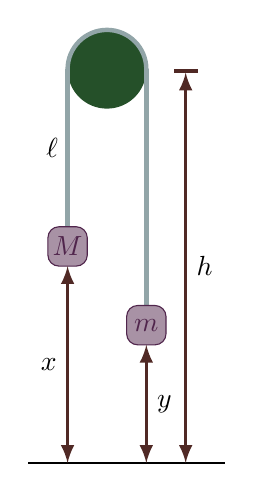
\begin{tikzpicture}
            \fill[highlight] (0, 0) circle [radius = 0.5cm];
            \draw[ultra thick, complementaryteal!50] (0.5, 0) -- ++ (0, -3);
            \draw[ultra thick, complementaryteal!50] (-0.5, 0) -- ++ (0, -2);
            \draw[ultra thick, complementaryteal!50] (0.5, 0) arc(0:180:0.5);
            \draw[rounded corners, complementarypurple, fill=complementarypurple!50] (0.25, -3) rectangle (0.75, -3.5) node[midway] {\(m\)};
            \draw[rounded corners, complementarypurple, fill=complementarypurple!50] (-0.25, -2) rectangle (-0.75, -2.5) node[midway] {\(M\)};
            \draw (-1, -5) -- (1.5, -5);
            \draw[complementaryred, <->, very thick] (0.5, -5) -- (0.5, -3.5) node[right, black, midway] {\(y\)};
            \draw[complementaryred, <->, very thick] (-0.5, -5) -- (-0.5, -2.5) node[left, black, midway] {\(x\)};
            \draw[complementaryred, <->|, very thick] (1, -5) -- (1, 0) node[right, black, midway] {\(h\)};
            \node[left] at (-0.5, -1) {\(\ell\)};
        \end{tikzpicture}
        \caption{Atwood's machine.}
        \label{fig:atwood machine}
    \end{figure}
    
    There are two degrees of freedom, we take them to be \(x\) and \(y\), the heights of \(M\) and \(m\) respectively, above some fixed floor a distance \(h\) below the pulley.
    There is one holonomic constraint:
    \begin{equation}
        x + y + \ell = 2h,
    \end{equation}
    where \(\ell\) is the length of the string\footnote{we can either assume the radius of the pulley is negligible or we can slightly redefine our coordinates to account for the part of the string that goes over the pulley.}.
    After applying this constraint we have one remaining degree of freedom.
    We take this to be \(x\).
    This lets us write
    \begin{equation}
        y = 2h - x - \ell.
    \end{equation}
    Differentiating this we have
    \begin{equation}
        \dot{y} = -\dot{x}.
    \end{equation}
    The total kinetic energy is just the kinetic energy of the two masses:
    \begin{equation}
        T = \frac{1}{2}M\dot{x}^2 + \frac{1}{2}m\dot{y}^2 = \frac{1}{2}M\dot{x}^2 + \frac{1}{2}m(-\dot{x})^2 = \frac{1}{2}(M + m)\dot{x}^2.
    \end{equation}
    The potential energy is gravitational potential energy of the two blocks, we define the floor as where the potential is zero.
    \begin{equation}
        V = Mgx + mgy = Mgx + mg(2h - x - \ell) = (M - m)gx + \text{constant}.
    \end{equation}
    Since we always differentiate the Lagrangian it is invariant under addition (or removal) of a constant term so we discard the constant.
    The Lagrangian for the system is then
    \begin{equation}
        \lagrangian = \frac{1}{2}(M - m)\dot{x}^2 - (M - m)gx.
    \end{equation}
    Hence,
    \begin{gather}
        \diffp{\lagrangian}{\dot{x}} = (M - m)\dot{x},\\
        \diffp{\lagrangian}{x} = -(M - m)g.
    \end{gather}
    Hence the equation of motion for the system is
    \begin{equation}
        (M - m)\ddot{x} = -(M - m)g \implies \ddot{x} = -\frac{M - m}{M + m}g.
    \end{equation}
    
    Notice that we don't have to consider the tension in the string, which is a real pain with the Newtonian derivation.
    
    \subsection{Atwood's Monkey}
    \defineindex{Atwood's monkey} is a modification of Atwood's machine where the mass \(M\) is replaced with a monkey of mass \(M\) which climbs up the rope at a known velocity, \(\dot{\varphi}(t)\), which is such that at time \(t\) the monkey is a distance \(\varphi(t)\) from the end of the rope.
    
    Again we initially have two degrees of freedom, \(x\) and \(y\), where now \(x\) is the distance of the monkey above the floor and \(y\) is still the height of \(m\).
    We have one holonomic constraint,
    \begin{equation}
        x + y + \ell - \varphi(t) = 2h.
    \end{equation}
    This allows us to eliminate \(y\):
    \begin{equation}
        y = 2h - x - \ell + \varphi(t).
    \end{equation}
    Differentiating this we now have
    \begin{equation}
        \dot{y} = -\dot{x} + \dot{\varphi}(t).
    \end{equation}
    The kinetic energy is then
    \begin{align}
        T &= \frac{1}{2}M\dot{x}^2 + \frac{1}{2}m\dot{y}^2\\
        &= \frac{1}{2}M\dot{x}^2 + \frac{1}{2}m(-\dot{x} + \dot{\varphi})^2\\
        &= \frac{1}{2}(M + m)\dot{x}^2 + \frac{1}{2}m\dot{\varphi}^2 - m\dot{x}\dot{\varphi}.
    \end{align}
    The potential energy is
    \begin{align}
        V &= Mgx + mgy\\
        &= Mgx + mg(2h - x - \ell + \varphi)\\
        &= (M - m)gx + mg\varphi + \text{constant}.
    \end{align}
    The Lagrangian is then
    \begin{equation}
        \lagrangian = \frac{1}{2}(M + m)\dot{x}^2 + \frac{1}{2}m\dot{\varphi}^2 - m\dot{x}\dot{\varphi} - (M - m)gx - mg\varphi.
    \end{equation}
    We then have
    \begin{gather}
        \diffp{\lagrangian}{\dot{x}} = (M + m)\dot{x} - m\dot{\varphi} \implies \diff*{\left( \diffp{\lagrangian}{\dot{x}} \right)}{t} = (M + m)\ddot{x} - m\ddot{\varphi},\\
        \diffp{\lagrangian}{x} = -(M - m)g.
    \end{gather}
    The equation of motion for the system is then
    \begin{equation}
        (M + m)\ddot{x} - m\ddot{\varphi} = -(M - m)g \implies \ddot{x} = -\frac{M - m}{M + m}g + \frac{m}{M + m}\ddot{\varphi}.
    \end{equation}
    We can integrate this to get
    \begin{equation}
        x(t) = -\frac{1}{2}\frac{M - m}{M + m}gt^2 + \frac{m}{M + m}\varphi(t) + At + B
    \end{equation}
    for constants of integration \(A\) and \(B\), which are fixed by the initial conditions.
    
    Notice that the monkey does work on the system and so energy is not conserved.
    
    \section{Particle and Wedge}
    Consider a particle on a smooth wedge, which in turn is on a smooth table.
    What is the acceleration of the wedge?
    Suppose the particle has mass \(m\), the wedge has mass \(M\), and the wedge angle is \(\varphi\).
    
    \begin{figure}
        \tikzsetnextfilename{block-wedge}
        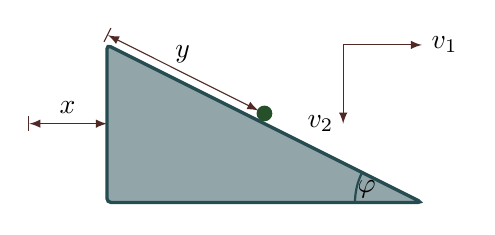
\begin{tikzpicture}
            \fill[complementaryteal!50, very thick, rounded corners=0.05cm] (0, 0) coordinate (C) -- (4, 0) coordinate (B) -- (0, 2) coordinate (A) -- cycle;
            \path pic [draw, "\(\varphi\)", angle radius=0.85cm, angle eccentricity=0.85, complementaryteal, thick, text=black] {angle};
            \draw[complementaryteal, very thick, rounded corners=0.05cm] (0, 0) -- (4, 0) -- (0, 2) -- cycle;
            \fill[highlight] (2, 1.13) circle [radius = 0.1cm];
            \draw[complementaryred, |<->] (0, 2.13) -- ++ (-26.6:2.15) node[midway, above, black] {\(y\)};
            \draw[complementaryred, |<->] (-1, 1) -- (0, 1) node[midway, above, black]  {\(x\)};
            \draw[complementaryred, <->] (4, 2) node[black, right] {\(v_1\)} -- (3, 2) -- (3, 1) node[black, left] {\(v_2\)};
        \end{tikzpicture}
        \caption{A particle on a wedge which is free to move.}
        \label{fig:particle wedge}
    \end{figure}
    
    There are two degrees of freedom.
    We choose them to be the position of the wedge and how far down the wedge the particle has slid.
    See \cref{fig:particle wedge}.
    Note that these are \emph{not} orthogonal.
    We have been asked to find out the acceleration of the wedge and we have chosen its position as one of our generalised coordinates.
    It is generally a good idea to have desired quantities as generalised coordinates.
    
    The kinetic energy has two contributions, first from the particle
    \begin{equation}
        \frac{1}{2}M\dot{x}^2,
    \end{equation}
    and from the particle,
    \begin{equation}
        \frac{1}{2}m(v_1^2 + v_2^2) = \frac{1}{2}m[(\dot{x} + \dot{y}\cos\varphi)^2 + (\dot{y}\sin\varphi)^2] = \frac{1}{2}m(\dot{x}^2 + \dot{y}^2 + 2\dot{x}\dot{y}\cos\varphi).
    \end{equation}
    The potential energy is provided by the particles gravitational potential energy, so its given by
    \begin{equation}
        V = -mgy\sin\varphi,
    \end{equation}
    taking the top of the ramp as zero potential energy.
    
    The Lagrangian for the system is
    \begin{equation}
        \lagrangian = \frac{1}{2}M\dot{x}^2 + \frac{1}{2}m(\dot{x}^2 + \dot{y}^2 + 2\dot{x}\dot{y}\cos\varphi) + mgy\sin\varphi.
    \end{equation}
    First consider \(x\):
    \begin{gather}
        \diffp{\lagrangian}{\dot{x}} = M\dot{x} + m\dot{x} + 2\dot{y}\cos\varphi \implies \diff*{\left( \diffp{\lagrangian}{\dot{x}} \right)}{t} = M\ddot{x} + m\ddot{x} + 2\ddot{y}\cos\varphi,\\
        \diffp{\lagrangian}{x} = 0.
    \end{gather}
    Hence
    \begin{equation}
        (M + m)\ddot{x} +m\ddot{y}\cos\varphi = 0.
    \end{equation}
    For \(y\) we get
    \begin{equation}
        \diffp{\lagrangian}{\dot{y}} = m\dot{y} + 2\dot{x}\cos\varphi \implies \diff*{\left( \diffp{\lagrangian}{\dot{y}} \right)}{t} = m\ddot{y} + 2\ddot{x}\cos\varphi,\\
        \diffp{\lagrangian}{y} = mg\sin\varphi,
    \end{equation}
    Hence
    \begin{equation}
        m\ddot{y} + 2\ddot{x}\cos\varphi = mg\sin\varphi.
    \end{equation}
    We now have two simultaneous equations in \(\ddot{x}\) and \(\ddot{y}\).
    Rearranging the first to give \(\ddot{y}\) and substituting into the second we can solve for \(\ddot{x}\) and we get
    \begin{equation}
        \ddot{x} = \frac{g\sin\varphi}{\cos\varphi - (m + M)\sec(\varphi)/m}.
    \end{equation}
    
    \section{Pendula}
    \subsection{Simple Pendulum}
    Consider a \defineindex{simple pendulum} consisting of a mass, \(m\), on the end of a light, rigid rod of length \(a\), fixed at the other end and constrained to move in a plane.
    Let \(\vartheta\) be the angle the pendulum makes to the vertical.
    
    \begin{figure}
        \tikzsetnextfilename{simple-pendulum}
        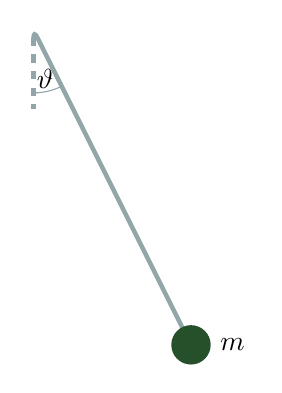
\begin{tikzpicture}
            \draw[ultra thick, complementaryteal!50, rounded corners=0.1cm] (2, -4) coordinate (C) -- (0, 0) coordinate (B) -- (0, -0.2) coordinate (A);
            \draw[ultra thick, complementaryteal!50, dashed] (0, -0.1) -- (0, -1);
            \fill[highlight] (2, -4) circle[radius=0.25cm];
            \path pic [draw, "\(\vartheta\)", angle radius=0.8cm, angle eccentricity=0.8, complementaryteal!50, text=black] {angle};
            \node[right] at (2.25, -4) {\(m\)};
        \end{tikzpicture}
        \caption{Simple pendulum.}
    \end{figure}
    
    The kinetic energy of the system is
    \begin{equation}
        T = \frac{1}{2}ma^2\dot{\vartheta}^2.
    \end{equation}
    The potential energy of the system is the gravitational potential energy of the bob.
    With a bit of trigonometry we can show that the distance of the pendulum bob below the attachment is \(a\cos\vartheta\), and hence the potential energy is
    \begin{equation}
        V = -mga\cos\vartheta.
    \end{equation}

    The Lagrangian of the system is
    \begin{equation}
        \lagrangian = \frac{1}{2}ma^2\dot{\vartheta}^2 + mga\cos\vartheta.
    \end{equation}
    Hence
    \begin{gather}
        \diffp{\lagrangian}{\dot{\vartheta}} = ma^2\dot{\vartheta} \implies \diff*{\left( \diffp{\lagrangian}{\dot{\vartheta}} \right)}{t} = ma^2\ddot{\vartheta},\\
        \diffp{\lagrangian}{\vartheta} = -mga\sin\vartheta.
    \end{gather}
    Hence the equation of motion for a pendulum is
    \begin{equation}
        ma^2\ddot{\vartheta} = -mga\sin\vartheta.
    \end{equation}
    With the small angle approximation we recover the familiar simple harmonic motion equation
    \begin{equation}
        \ddot{\vartheta} = -\omega^2\vartheta
    \end{equation}
    with \(\omega = \sqrt{g/a}\).
    
    \subsection{Spherical Pendulum}
    The \defineindex{spherical pendulum} is like the simple pendulum but no longer restricted to swing in a plane.
    Instead we have an extra degree of freedom, which we take to be the angle, \(\varphi\), about the vertical through which the pendulum swings.
    
    \begin{figure}
        \tikzsetnextfilename{spherical-pendulum}
        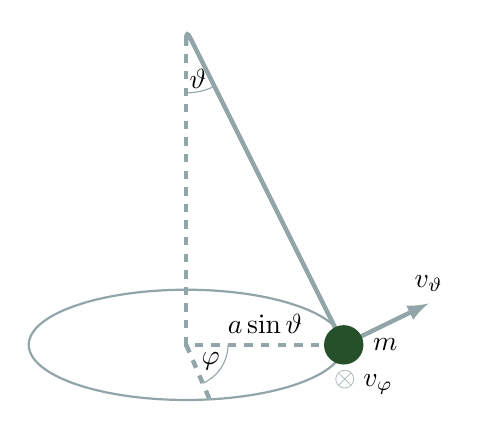
\begin{tikzpicture}
            \draw[thick, complementaryteal!50] (0, -4) circle [x radius = 2cm, y radius = 0.7cm];
            \draw[->, ultra thick, complementaryteal!50] (2, -4) -- ++ (26:1.2) node[above, black] {\(v_\vartheta\)};
            \draw[ultra thick, complementaryteal!50, rounded corners=0.1cm] (2, -4)
            coordinate (C) -- (0, 0) coordinate (B) -- (0, -0.2) coordinate (A);
            \draw[ultra thick, complementaryteal!50, dashed] (0, -0.1) -- (0, -4) -- (2, -4) node[midway, above, black] {\(a\sin\vartheta\)};
            \fill[highlight] (2, -4) circle[radius=0.25cm];
            \path pic [draw, "\(\vartheta\)", angle radius=0.8cm, angle eccentricity=0.8, complementaryteal!50, text=black] {angle};
            \draw[complementaryteal!50, ultra thick, dashed] (0, -4) coordinate (B) -- (0.3, -4.7) coordinate (A);
            \path pic [draw, "\(\varphi\)", complementaryteal!50, text=black, angle radius=0.53cm, angle eccentricity=0.7] {angle};
            \node[right] at (2.25, -4) {\(m\)};
            \node[below] at (2.25, -4.2) {\(\textcolor{complementaryteal!50}{\otimes}\;v_\varphi\)};
        \end{tikzpicture}
        \caption{Spherical Pendulum.}
    \end{figure}
    
    The kinetic energy of the pendulum is
    \begin{equation}
        T = \frac{1}{2}m(v_{\vartheta}^2 + v_{\varphi}^2)
    \end{equation}
    where \(v_{\vartheta} = a\dot{\vartheta}\) and \(v_{\varphi} = a\dot{\varphi}\sin\vartheta\), since \(a\sin\vartheta\) is the radius of the circle defined by \(\vartheta\) being constant and varying \(\varphi\).
    That is
    \begin{equation}
        T = \frac{1}{2}ma^2\dot{\varphi}^2\sin^2\vartheta + \frac{1}{2}ma^2\dot{\vartheta}^2.
    \end{equation}
    The potential energy is the same as for the simple pendulum,
    \begin{equation}
        V = -mga\cos\vartheta.
    \end{equation}

    The Lagrangian for the system is
    \begin{equation}
        \lagrangian = \frac{1}{2}ma^2\dot{\varphi}^2\sin^2\vartheta + \frac{1}{2}ma^2\dot{\vartheta}^2 + mga\cos\vartheta.
    \end{equation}
    Considering \(\vartheta\) we have
    \begin{gather}
        \diffp{\lagrangian}{\dot{\vartheta}} = ma^2\dot{\vartheta} \implies \diff*{\left( \diffp{\lagrangian}{\dot{\vartheta}} \right)}{t} = ma^2\ddot{\vartheta},\\
        \diffp{\lagrangian}{\vartheta} = ma^2\dot{\varphi}^2\sin\vartheta\cos\vartheta - mga\sin\vartheta
    \end{gather}
    giving the equation of motion
    \begin{equation}\label{eqn:spheirical pendulum theta eom}
        ma^2\ddot{\vartheta} = ma^2\dot{\varphi}^2\sin\vartheta\cos\vartheta - mgas\sin\vartheta.
    \end{equation}
    
    Now considering \(\varphi\) we have
    \begin{gather}
        \diffp{\lagrangian}{\dot{\varphi}} = ma^2\dot\varphi\sin^2\vartheta \implies \diff*{\left( \diffp{\lagrangian}{\dot{\varphi}} \right)}{t} = ma^2\ddot{\varphi}\sin^2\vartheta +2ma^2\dot{\varphi}\dot{\vartheta}\sin\vartheta\cos\vartheta\\
        \diffp{\lagrangian}{\varphi} = 0.
    \end{gather}
    Hence the equation of motion for \(\varphi\) is
    \begin{equation}\label{eqn:spherical pendulum phi eom}
        ma^2\ddot{\varphi}\sin^2\vartheta +2ma^2\dot{\varphi}\dot{\vartheta}\sin\vartheta\cos\vartheta = 0.
    \end{equation}
    
    We have two coupled differential equations.
    Integrating \cref{eqn:spherical pendulum phi eom} gives
    \begin{equation}
        ma^2\dot{\varphi}\sin^2\vartheta = \text{constant}.
    \end{equation}
    We can identify this constant as \(L_z\), the \(z\) component of the angular momentum.
    This equation implies conservation of angular momentum about the vertical axis.
    
    We can then substitute in \(\dot{\varphi}\) into \cref{eqn:spheirical pendulum theta eom} in terms of the angular momentum giving
    \begin{equation}
        ma^2\ddot{\vartheta} = ma^2\sin\vartheta\cos\vartheta \left( \frac{L_z}{a^2\sin^2\vartheta} \right)^2 - mag\sin\vartheta.
    \end{equation}
    Multiplying through by \(\dot{\vartheta}\) we can integrate both sides with respect to \(t\) which gives
    \begin{equation}
        \frac{1}{2}ma^2\dot{\vartheta}^2 = mga\cos\vartheta - \frac{L_z^2}{2ma^2\sin^2\vartheta} + \text{constant}.
    \end{equation}
    Rearranging we get
    \begin{equation}
        \frac{1}{2}ma^2\dot{\vartheta}^2 + \frac{L_z^2}{2ma^2\sin^2\vartheta} - mga\cos\vartheta = \text{constant}.
    \end{equation}
    We can identify this constant as the energy, \(E\), in particular the first two terms are the \(\vartheta\) and \(\varphi\) contributions to the kinetic energy and the last term is the potential energy.
    
    \subsubsection{Notes}
    Conservation of \(L_z\) arises because the Lagrangian is invariant under rotations about the \(z\) axis, we can see this because the Lagrangian is independent of \(\varphi\).
    This gives us a general rule
    \begin{equation}
        \diffp{\lagrangian}{q} = 0 \implies \diffp{\lagrangian}{\dot{q}} = \text{constant}.
    \end{equation}

    We will also show later that time independence of the Lagrangian (or equivalently invariance under time translations) implies conservation of energy.
    In fact every symmetry (i.e. something that leaves the Lagrangian invariant) implies a conservation law and vice versa.
    This is \defineindex{Noether's theorem}, a concept we will return to later.
    
    In this case it may have been easier to give the conservation laws by inspection:
    \begin{align}
        L_z &= ma^2 \dot{\varphi} \sin^2\vartheta = \text{constant},\\
        E &= \frac{1}{2}ma^2\dot{\vartheta}^2 + \frac{L_z^2}{2ma^2\sin^2\vartheta} - mga\cos\vartheta = \text{constant}.
    \end{align}
    This gives us two first order differential equations which are the two \define{first integrals}\index{first integral} of Lagrange's equations.
    Each symmetry will give a first integral, which gets us a fair way to solving the system.
    
    If there are as many symmetries as degrees of freedom, as is the case here, then we can often write down a set of first order differential equations like this without having to consider Lagrange's equations at all.
    We call systems where this is possible \defineindex{integrable}.
    
    %Appendicies
    \appendixpage
    \begin{appendices}
        \chapter{Differential Equations}
Many of the equations of motion we will derive are second order linear ordinary differential equations of the form
\begin{equation}
    ay''(x) + by'(x) + cy(x) = f(x)
\end{equation}
for some constants \(a\), \(b\), and \(c\), and functions \(y\) and \(f\).
There is a general procedure for solving such equations.
\begin{enumerate}
    \item First define the homogenous equation
    \begin{equation}
        ay''(x) + by'(x) + cy(x) = 0.
    \end{equation}
    This is important since if \(y_1\) is a solution to the homogeneous equation and \(y_p\) is a solution to the inhomogeneous equation then \(y_p + \lambda y_1\) with \(\lambda\) being a constant, is a solution to the original inhomogeneous equation also.
    The most general solution is the solution to the inhomogeneous equation and a linear combination of solutions to the homogenous equation.
    The number of solutions to the homogenous equation is equal to the order of the equation, so for our purposes 2.
    \item Solve the homogenous equation.
    This is usually done by making a guess and substituting into the homogenous equation and solving for any unknowns in the guess.
    The most common guess is of the form \(\e^{mx}\).
    If we make this guess after substitution we have
    \begin{equation}
        (am^2 + bm + c)\e^{mx} = 0.
    \end{equation}
    Since \(\e^{mx} \ne 0\) we must therefore have that the quadratic in \(m\) is zero.
    This gives us two values for \(m\), \(m_1\) and \(m_2\).
    If \(m_1 \ne m_2\) then we define
    \begin{equation}
        y_1(x) = \e^{m_1x}, \qqand y_2(x) = \e^{m_2x}.
    \end{equation}
    If \(m_1 = m_2\) then instead define
    \begin{equation}
        y_1(x) = \e^{m_1x}, \qqand y_2(x) = x\e^{m_1x}.
    \end{equation}
    Occasionally other guesses, such as trig functions, make more sense, particularly if there are no first derivatives in the equation.
    
    \item Returning to the inhomogeneous equation we now need to find a solution, \(y_p\), of course if the original equation was inhomogeneous then this step can be skipped.
    We again do this by guessing.
    The exact guess depends on the form of \(f\) but some common choices are given in \cref{tab:common guesses for differential equation}.
    \begin{table}
        \caption{Common guesses to solve the inhomogeneous differential equation \(ay''(x) + by'(x) + cy(x) = f(x)\) for different functions \(f\).}
        \label{tab:common guesses for differential equation}
        \begin{tabular}{cc}
            \toprule
            Form of \(f\) & Suggestion for \(y_p\)\\\midrule
            Constant, \(k\) & Constant \(k/c\)\\
            Polynomial in \(x\) & Polynomial in \(x\)\\
            \(ke^{\alpha x}\) & \(A e^{\alpha x}\)\\
            \(\sin(\alpha x)\) and/or \(\cos(\alpha x)\) & \(A\sin(\alpha x) + B\cos(\alpha x)\)\\\bottomrule
        \end{tabular}
    \end{table}
    Once you have chosen a function substitute it in and see if it is valid.
    
    \item If you have no boundary conditions then you are done.
    The solution is
    \begin{equation}
        y(x) = y_p(x) + \sum_i\lambda_i y_i(x)
    \end{equation}
    where \(y_i\) are solutions to the homogeneous equation.
    If you have boundary conditions then substitute them into this equation and solve for \(\lambda_i\).
\end{enumerate}

\begin{exm}{}{}
    Suppose we wish to solve
    \begin{equation}
        y''(x) + 4y'(x) + 4y(x) = \sin(3x),
    \end{equation}
    with the boundary conditions \(y(0) = 10\) and \(y'(0) = 0\).
    
    We start by defining the homogeneous equation
    \begin{equation}
        y''(x) + 4y'(x) + 4y(x) = 0.
    \end{equation}
    We propose that \(\e^{mx}\) is a solution to this.
    Substituting this in we find
    \begin{equation}
        (m^2 + 4m^2 + 4)\e^{mx} = 0.
    \end{equation}
    The quadratic has one repeated root \(m = -2\) and so our solutions to the homogenous equation are
    \begin{equation}
        y_1(x) = \e^{-2x}, \qqand y_2(x) = x\e^{-2x}.
    \end{equation}
    
    In this case \(f(x) = \sin(3x)\) and so we try a solution of the form
    \begin{equation}
        y_p(x) = A\sin(3x) + B\cos(3x).
    \end{equation}
    Substituting this into our original equation we have
    \begin{multline}
        -9A\sin(3x) -9B\cos(3x) + 12A\cos(3x) - 12B\sin(3x)\\ + 4A\sin(3x) + 4B\cos(3x)\\= -(5A + 12B)\sin(3x) + (12A - 5B)\cos(3x).
    \end{multline}
    In order for this to be equal to \(\sin(3x)\) we require that
    \begin{equation}
        5A + 12B = -1, \qqand 12A - 5B = 0.
    \end{equation}
    Solving these simultaneous equations gives us
    \begin{equation}
        A = -\frac{5}{169}, \qqand B = -\frac{12}{169}.
    \end{equation}
    Hence our solution is
    \begin{equation}
        y_p(x) = -\frac{5}{169} \sin(3x) - \frac{12}{169} \cos(3x).
    \end{equation}
    
    The general solution is then
    \begin{equation}
        y(x) = -\frac{5}{169} \sin(3x) - \frac{12}{169} \cos(3x) + \lambda_1\e^{-2x} + \lambda_2x\e^{-2x}.
    \end{equation}
    Substituting for our first initial condition, \(y(0) = 10\), we have
    \begin{equation}
        y(0) = -\frac{12}{169} + \lambda_1 = 10 \implies \lambda_1 = \frac{1702}{169}.
    \end{equation}
    The second initial condition, \(y'(0) = 0\), gives us
    \begin{equation}
        y'(0) = -\frac{15}{169} - 2\frac{1702}{169} - 2\lambda_2 = 0 \implies \lambda_2 = -\frac{263}{26}.
    \end{equation}
    Hence our final solution is
    \begin{equation}
        y(x) = -\frac{5}{169} \sin(3x) - \frac{12}{169} \cos(3x) + \frac{1702}{169}\e^{-2x} - \frac{263}{26}x\e^{-2x}.
    \end{equation}
\end{exm}

    \end{appendices}
    
    \backmatter
    \renewcommand{\glossaryname}{Acronyms}
    \printglossary[acronym]
    \printindex
\end{document}
